% =============================================================================
%              Chapter 2: Requirements Specification and Analysis
% =============================================================================



% ==========================================================
% Pending Missing Visual Assets
% ==========================================================
\subsection{Pending Missing Visual Assets}

% TODO: Required Asset Name: WBS Diagram
% Asset Type: Missing Technical Visual Asset
% Status: Pending Asset Collection
\begin{figure}[H]
    \centering
    \includegraphics[width=0.8\textwidth]{figures/chapter2/wbs_diagram_formal.png}
    \caption{[Placeholder] WBS Diagram}
    \label{fig:placeholder_wbs_diagram_formal}
\end{figure}

[PLACEHOLDER EXPLANATION]: This section serves as a 4-to-5 line explanatory paragraph that will describe the visual asset presented above. It will comprehensively detail the purpose, underlying structure, and operational significance of the diagram, chart, or screenshot. By providing this extensive textual context, the report will ensure that readers fully understand the specific components, workflows, and technical details illustrated in the figure. (This text will be manually updated by the user once the final image is inserted).

% TODO: Required Asset Name: Gantt Chart
% Asset Type: Missing Technical Visual Asset
% Status: Pending Asset Collection
\begin{figure}[H]
    \centering
    \includegraphics[width=0.8\textwidth]{figures/chapter2/gantt_chart_formal.png}
    \caption{[Placeholder] Gantt Chart}
    \label{fig:placeholder_gantt_chart_formal}
\end{figure}

[PLACEHOLDER EXPLANATION]: This section serves as a 4-to-5 line explanatory paragraph that will describe the visual asset presented above. It will comprehensively detail the purpose, underlying structure, and operational significance of the diagram, chart, or screenshot. By providing this extensive textual context, the report will ensure that readers fully understand the specific components, workflows, and technical details illustrated in the figure. (This text will be manually updated by the user once the final image is inserted).

\setcounter{chapter}{2}
\setcounter{figure}{0}
\setcounter{table}{0}
\chapter*{Chapter 2}
\markboth{Requirement Specification and Analysis}{Requirement 
Specification and Analysis} 
\section{Requirement Specification and Analysis}

This chapter describes the functional requirements of the Smart AI 
Powered Agriculture System in terms of epics, user stories, test 
cases, user interface design, and a traceability matrix 
\cite{sommerville2016software}.

\subsection{Epics}

Epics are large, high-level features that represent significant 
functionalities of the system \cite{ferreira2022userstories}. Each 
epic is later broken down into multiple user stories.

\subsubsection{E1: User Authentication and Profile Management}

\textbf{Description:} As a farmer or administrator, the user wants 
to securely log in, register, and manage their profile so that data 
and farm configurations remain private and secure \cite{jwtmqtt2019}.

\subsubsection{E2: Real-Time Sensor Data Monitoring}

\textbf{Description:} As a farmer, the user wants to monitor 
real-time environmental data (soil moisture, temperature, humidity) 
from the fields so that informed decisions can be made about crop 
care \cite{ncbi2023iot}.

\subsubsection{E3: Intelligent Irrigation Control}

\textbf{Description:} As a farmer, the user wants to control 
irrigation systems manually or set automatic triggers based on sensor 
thresholds so that water usage is optimized and crops receive adequate 
hydration \cite{iotsmartag2024}.

\subsubsection{E4: AI-Driven Crop Recommendations}

\textbf{Description:} As a farmer, the user wants to receive 
AI-generated crop recommendations based on soil and weather analysis 
so that yield can be maximized and the most suitable crops for the 
season can be selected \cite{musanase2023data}.

\subsubsection{E5: Alerting and Notification System}

\textbf{Description:} As a farmer, the user wants to receive 
immediate alerts about critical conditions (e.g., low soil moisture, 
sensor failure) so that timely corrective actions can be taken to 
prevent crop damage \cite{saha2024automated}.

\subsubsection{E6: Historical Data Analytics and Visualization}

\textbf{Description:} As a farmer, the user wants to view historical 
trends and graphical visualizations of farm data so that long-term 
patterns can be analyzed and farming strategies improved 
\cite{ncbi2023iot}.

\subsection{User Stories}

To bridge the gap between high-level project goals and actionable technical 
development, each Epic is decomposed into smaller, discrete User Stories 
\cite{ferreira2022userstories}. These stories define the exact interaction 
boundaries between the end-user (farmer or administrator) and the system 
components (e.g., the Flutter application, the Node.js backend, or the 
ESP32 hardware). Each story is accompanied by explicit acceptance criteria, 
forming the foundational contract for the subsequent system testing phase.

\subsubsection{Epic E1: User Authentication and Profile Management}

\paragraph{E1-US1: User Registration} As a new user, the user wants 
to create an account using email and phone number so that system 
features can be accessed.

\textbf{Acceptance Criteria:}
\begin{itemize}[noitemsep]
    \item Given the user is on the registration screen,
    \item When valid name, email, phone, and password are entered,
    \item Then the system should create a new account and redirect 
    to the login page.
\end{itemize}

\paragraph{E1-US2: Secure Login} As a registered user, the user 
wants to log in using credentials so that the personal dashboard can 
be accessed \cite{jwtauth2017}.

\textbf{Acceptance Criteria:}
\begin{itemize}[noitemsep]
    \item Given the user has a valid account,
    \item When the correct email and password are entered,
    \item Then the system should authenticate the user and grant 
    access to the dashboard.
\end{itemize}

\paragraph{E1-US3: Profile Management} As a user, the user wants to 
update personal information and change the password so that account 
details remain current and secure.

\textbf{Acceptance Criteria:}
\begin{itemize}[noitemsep]
    \item Given the user is logged in,
    \item When the user navigates to profile settings and updates 
    the phone number,
    \item Then the system should save the changes and display a 
    success message.
\end{itemize}

\subsubsection{Epic E2: Real-Time Sensor Data Monitoring}

\paragraph{E2-US1: View Field Overview}

\textbf{Description:} As a farmer, the user wants to see a list of 
all fields with their current status so that the overall farm health 
can be assessed quickly \cite{saha2024automated}.

\textbf{Acceptance Criteria:}
\begin{itemize}[noitemsep]
    \item Given the user is on the dashboard,
    \item When the page loads,
    \item Then the system should display all registered fields with 
    summary indicators such as ``Healthy'' or ``Needs Water''.
\end{itemize}

\paragraph{E2-US2: Detailed Sensor Readings}

\textbf{Description:} As a farmer, the user wants to view specific 
readings from individual sensors (e.g., Sensor ID 14) so that issues 
in specific areas can be pinpointed \cite{ncbi2023iot}.

\textbf{Acceptance Criteria:}
\begin{itemize}[noitemsep]
    \item Given the user selects a specific field,
    \item When a sensor node is tapped,
    \item Then the system should show the latest values for soil 
    moisture, temperature, and humidity.
\end{itemize}

\paragraph{E2-US3: Sensor Status Monitoring}

\textbf{Description:} As a farmer, the user wants to know if a 
sensor is offline or has low battery so that maintenance can be 
performed.

\textbf{Acceptance Criteria:}
\begin{itemize}[noitemsep]
    \item Given a sensor has stopped sending data,
    \item When the user views the sensor list,
    \item Then the system should display an ``Offline'' status 
    indicator next to that sensor.
\end{itemize}

\subsubsection{Epic E3: Intelligent Irrigation Control}

\paragraph{E3-US1: Manual Irrigation Toggle}

\textbf{Description:} As a farmer, the user wants to remotely turn 
the water pump on or off so that the field can be irrigated 
immediately when needed \cite{iotsmartag2024}.

\textbf{Acceptance Criteria:}
\begin{itemize}[noitemsep]
    \item Given the irrigation system is connected,
    \item When the user presses the ``Start Irrigation'' button,
    \item Then the system should send a command to the actuator and 
    update the status to ``Irrigating''.
\end{itemize}

\paragraph{E3-US2: Threshold-Based Automation}

\textbf{Description:} As a farmer, the user wants to set a soil 
moisture threshold (e.g., 30\%) so that the system automatically 
irrigates when the soil becomes too dry \cite{garcia2020iot}.

\textbf{Acceptance Criteria:}
\begin{itemize}[noitemsep]
    \item Given the automation mode is enabled,
    \item When soil moisture drops below the defined threshold,
    \item Then the system should automatically trigger the irrigation 
    pump without user intervention.
\end{itemize}

\paragraph{E3-US3: Irrigation Logging}

\textbf{Description:} As a farmer, the user wants to see a history 
of irrigation events so that water usage can be tracked.

\textbf{Acceptance Criteria:}
\begin{itemize}[noitemsep]
    \item Given an irrigation cycle has completed,
    \item When the user views the irrigation logs,
    \item Then the system should list the start time, end time, and 
    total duration of each event.
\end{itemize}

\subsubsection{Epic E4: AI-Driven Crop Recommendations}

\paragraph{E4-US1: Request Crop Recommendation}

\textbf{Description:} As a farmer, the user wants to request a crop 
recommendation based on the field's current soil data so that the 
most viable crop can be planted \cite{musanase2023data}.

\textbf{Acceptance Criteria:}
\begin{itemize}[noitemsep]
    \item Given the user is on the recommendation screen,
    \item When the ``Analyze Field'' button is clicked,
    \item Then the system should process the soil parameters and 
    display a recommended crop (e.g., ``Wheat'').
\end{itemize}

\paragraph{E4-US2: View Recommendation Confidence}

\textbf{Description:} As a farmer, the user wants to see the 
confidence score of the AI prediction so that trust in the 
recommendation can be established \cite{akkem2024enhancing}.

\textbf{Acceptance Criteria:}
\begin{itemize}[noitemsep]
    \item Given a recommendation is generated,
    \item When the result is displayed,
    \item Then the system should show a percentage confidence score 
    (e.g., ``85\% Confidence'').
\end{itemize}

\paragraph{E4-US3: Accept Recommendation}

\textbf{Description:} As a farmer, the user wants to mark a 
recommendation as ``Accepted'' so that the system tracks what has 
actually been planted.

\textbf{Acceptance Criteria:}
\begin{itemize}[noitemsep]
    \item Given a recommendation is displayed,
    \item When the user clicks ``Accept'',
    \item Then the field's current crop status should be updated to 
    match the recommendation.
\end{itemize}

\subsubsection{Epic E5: Alerting and Notification System}

\paragraph{E5-US1: Critical Threshold Alerts}

\textbf{Description:} As a farmer, the user wants to receive a 
notification when soil moisture is critically low so that crops do 
not die due to lack of water \cite{khawas2018firebase}.

\textbf{Acceptance Criteria:}
\begin{itemize}[noitemsep]
    \item Given the soil moisture is below the critical limit,
    \item When the sensor transmits the data,
    \item Then the system should generate a ``Critical Alert'' and 
    notify the user.
\end{itemize}

\paragraph{E5-US2: View Unread Alerts}

\textbf{Description:} As a farmer, the user wants to see a badge 
count of unread alerts so that any missed information is visible.

\textbf{Acceptance Criteria:}
\begin{itemize}[noitemsep]
    \item Given there are new alerts,
    \item When the user opens the app,
    \item Then the notification icon should show a badge with the 
    number of unread items.
\end{itemize}

\paragraph{E5-US3: Resolve Alerts}

\textbf{Description:} As a farmer, the user wants to mark an alert 
as resolved so that the notification feed can be cleared.

\textbf{Acceptance Criteria:}
\begin{itemize}[noitemsep]
    \item Given an active alert exists,
    \item When the user clicks ``Mark as Resolved'',
    \item Then the alert should be moved to the history archive and 
    its status updated.
\end{itemize}

\subsubsection{Epic E6: Historical Data Analytics and Visualization}

\paragraph{E6-US1: View Moisture Trends}

\textbf{Description:} As a farmer, the user wants to see a line 
graph of soil moisture over the last week so that drying patterns 
can be understood \cite{saha2024automated}.

\textbf{Acceptance Criteria:}
\begin{itemize}[noitemsep]
    \item Given historical data exists,
    \item When the user selects the ``Weekly View'' on the chart,
    \item Then the system should render a line graph showing moisture 
    levels over the past 7 days.
\end{itemize}

\paragraph{E6-US2: Export Data}

\textbf{Description:} As a farmer, the user wants to export farm 
data so that offline records can be kept.

\textbf{Acceptance Criteria:}
\begin{itemize}[noitemsep]
    \item Given the user is on the analytics screen,
    \item When the ``Export'' button is clicked,
    \item Then the system should generate a downloadable report 
    (e.g., CSV or PDF).
\end{itemize}

\paragraph{E6-US3: Compare Fields}

\textbf{Description:} As a farmer, the user wants to compare the 
water usage of two different fields so that inefficiencies can be 
identified.

\textbf{Acceptance Criteria:}
\begin{itemize}[noitemsep]
    \item Given the user selects two fields,
    \item When the ``Compare'' option is chosen,
    \item Then the system should display side-by-side statistics for 
    both fields.
\end{itemize}

\subsection{Test-cases}

To ensure rigorous validation of the developed system against the defined 
requirements, this section outlines the formal test cases mapped directly 
to the user stories \cite{tahir2019traceability}. Rather than relying 
solely on ad-hoc manual testing, these test cases define deterministic 
inputs—such as simulated ADC thresholds or mocked REST API payloads—and 
the exact expected state changes within the database or firmware. 
The tables below document the objective, preconditions, inputs, and 
actual validated outcomes for each core module.

\subsubsection{Test Case 1 --- Verify User Registration with Valid 
Data}

This test case verifies the user registration process. It checks 
whether the system correctly accepts valid user details, creates a 
new user account, stores the information in the database, and 
redirects the user to the login page successfully.

\begin{longtable}{|p{4cm}|p{8cm}|}
\caption{Verify User Registration with Valid Data}
\label{tab:tc_registration} \\
\hline
\textbf{Test ID} & TC-E1-US1-01 \\ \hline
\textbf{User Story ID} & E1-US1 \\ \hline
\textbf{Module} & User Authentication and Registration \\ \hline
\textbf{Test Case Description} & Verify that a new user can 
successfully register using valid credentials and personal 
information. \\ \hline
\textbf{Preconditions} & User is on the registration screen and 
backend server is operational. \\ \hline
\textbf{Test Inputs} &
Name = ``Ali Khan'' \newline
Email = ``ali@test.com'' \newline
Phone = ``+923001234567'' \newline
Password = ``Pass123'' \\ \hline
\textbf{Expected Result} & A new user account should be created 
successfully in the \texttt{users} table and the user should be 
redirected to the login page. \\ \hline
\textbf{Actual Result} & User account was created successfully and 
redirected to the login page correctly. \\ \hline
\textbf{Status} & Pass \\ \hline
\end{longtable}

\subsubsection{Test Case 2 --- Verify Login with Valid Credentials}

This test case validates the login functionality and ensures that a 
registered user can access the dashboard using valid credentials 
\cite{jwtauth2017}.

\begin{longtable}{|p{4cm}|p{8cm}|}
\caption{Verify Login with Valid Credentials}
\label{tab:tc_login} \\
\hline
\textbf{Test ID} & TC-E1-US2-01 \\ \hline
\textbf{User Story ID} & E1-US2 \\ \hline
\textbf{Module} & User Authentication \\ \hline
\textbf{Test Case Description} & Verify that a registered user can 
log into the system successfully using valid credentials. \\ \hline
\textbf{Preconditions} & User account already exists in the system 
database. \\ \hline
\textbf{Test Inputs} &
Email = ``ali@test.com'' \newline
Password = ``Pass123'' \\ \hline
\textbf{Expected Result} & System authenticates the user, generates 
JWT token, and redirects to dashboard with HTTP 200 OK response. 
\\ \hline
\textbf{Actual Result} & User was authenticated successfully and 
dashboard loaded correctly with valid JWT token. \\ \hline
\textbf{Status} & Pass \\ \hline
\end{longtable}

\subsubsection{Test Case 3 --- Verify Profile Management}

This test case verifies that a logged-in user can update profile 
information successfully.

\begin{longtable}{|p{4cm}|p{8cm}|}
\caption{Verify Profile Management}
\label{tab:tc_profile} \\
\hline
\textbf{Test ID} & TC-E1-US3-01 \\ \hline
\textbf{User Story ID} & E1-US3 \\ \hline
\textbf{Module} & Profile Management \\ \hline
\textbf{Test Case Description} & Verify that the user can update 
personal profile information successfully. \\ \hline
\textbf{Preconditions} & User is logged in and profile screen is 
accessible. \\ \hline
\textbf{Test Inputs} &
Updated Phone = ``+923009876543'' \\ \hline
\textbf{Expected Result} & Updated profile information should be 
saved in the \texttt{users} table and success message should be 
displayed. \\ \hline
\textbf{Actual Result} & Profile information was updated successfully 
and success message was displayed. \\ \hline
\textbf{Status} & Pass \\ \hline
\end{longtable}

\subsubsection{Test Case 4 --- Verify Field Overview Display}

This test case verifies that the dashboard displays all registered 
fields with their current status.

\begin{longtable}{|p{4cm}|p{8cm}|}
\caption{Verify Field Overview Display}
\label{tab:tc_field_overview} \\
\hline
\textbf{Test ID} & TC-E2-US1-01 \\ \hline
\textbf{User Story ID} & E2-US1 \\ \hline
\textbf{Module} & Real-Time Sensor Data Monitoring \\ \hline
\textbf{Test Case Description} & Verify that all registered fields 
are displayed on the dashboard with their current status. \\ \hline
\textbf{Preconditions} & User is logged in and fields are registered 
in the system. \\ \hline
\textbf{Test Inputs} & User opens the dashboard screen. \\ \hline
\textbf{Expected Result} & Dashboard should display all registered 
fields with status indicators such as ``Healthy'' or ``Needs 
Water''. \\ \hline
\textbf{Actual Result} & Registered fields were displayed 
successfully with correct status indicators. \\ \hline
\textbf{Status} & Pass \\ \hline
\end{longtable}

\subsubsection{Test Case 5 --- Verify Real-Time Data Display}

This test case verifies that real-time sensor readings are correctly 
displayed on the dashboard interface \cite{ncbi2023iot}.

\begin{longtable}{|p{4cm}|p{8cm}|}
\caption{Verify Real-Time Data Display}
\label{tab:tc_realtime} \\
\hline
\textbf{Test ID} & TC-E2-US2-01 \\ \hline
\textbf{User Story ID} & E2-US2 \\ \hline
\textbf{Module} & Real-Time Monitoring \\ \hline
\textbf{Test Case Description} & Verify that the latest sensor 
readings are correctly displayed on the user interface. \\ \hline
\textbf{Preconditions} & ESP32 device is connected and sending 
telemetry to backend server. \\ \hline
\textbf{Test Inputs} &
Sensor ID = 14 \newline
Moisture = 45\% \newline
Temperature = 30$^{\circ}$C \\ \hline
\textbf{Expected Result} & Dashboard should display updated moisture 
and temperature values matching the sensor readings stored in the 
database. \\ \hline
\textbf{Actual Result} & Dashboard displayed ``Moisture: 45\%'' and 
``Temperature: 30$^{\circ}$C'' correctly. \\ \hline
\textbf{Status} & Pass \\ \hline
\end{longtable}

\subsubsection{Test Case 6 --- Verify Sensor Status Monitoring}

This test case verifies that the system detects and displays sensor 
status correctly.

\begin{longtable}{|p{4cm}|p{8cm}|}
\caption{Verify Sensor Status Monitoring}
\label{tab:tc_sensor_status} \\
\hline
\textbf{Test ID} & TC-E2-US3-01 \\ \hline
\textbf{User Story ID} & E2-US3 \\ \hline
\textbf{Module} & Sensor Status Monitoring \\ \hline
\textbf{Test Case Description} & Verify that the system displays 
offline status when a sensor stops sending data. \\ \hline
\textbf{Preconditions} & Sensor is registered in the system and 
dashboard is accessible. \\ \hline
\textbf{Test Inputs} & Sensor ID = 14 stops sending telemetry 
data. \\ \hline
\textbf{Expected Result} & System should mark the sensor status as 
``Offline'' on the dashboard or sensor detail page. \\ \hline
\textbf{Actual Result} & Sensor status changed to ``Offline'' 
successfully when telemetry was not received. \\ \hline
\textbf{Status} & Pass \\ \hline
\end{longtable}

\subsubsection{Test Case 7 --- Verify Manual Pump Start}

This test case verifies the manual irrigation control functionality 
from the mobile application \cite{iotsmartag2024}.

\begin{longtable}{|p{4cm}|p{8cm}|}
\caption{Verify Manual Pump Start}
\label{tab:tc_pump} \\
\hline
\textbf{Test ID} & TC-E3-US1-01 \\ \hline
\textbf{User Story ID} & E3-US1 \\ \hline
\textbf{Module} & Irrigation Control System \\ \hline
\textbf{Test Case Description} & Verify that the irrigation pump 
starts successfully when triggered manually by the user. \\ \hline
\textbf{Preconditions} & ESP32 device and relay module are connected 
and operational. \\ \hline
\textbf{Test Inputs} & User clicks ``Start Irrigation'' button for 
Field ID = 6. \\ \hline
\textbf{Expected Result} & System should activate the relay, update 
pump status to ``ON'', and create a new irrigation log entry. \\ 
\hline
\textbf{Actual Result} & Pump activated successfully and irrigation 
status updated correctly in the application. \\ \hline
\textbf{Status} & Pass \\ \hline
\end{longtable}

\subsubsection{Test Case 8 --- Verify Automatic Trigger on Low 
Moisture}

This test case validates the automatic irrigation functionality 
based on soil moisture thresholds \cite{garcia2020iot}.

\begin{longtable}{|p{4cm}|p{8cm}|}
\caption{Verify Automatic Trigger on Low Moisture}
\label{tab:tc_auto} \\
\hline
\textbf{Test ID} & TC-E3-US2-01 \\ \hline
\textbf{User Story ID} & E3-US2 \\ \hline
\textbf{Module} & Automated Irrigation Control \\ \hline
\textbf{Test Case Description} & Verify that the system 
automatically starts irrigation when soil moisture falls below the 
configured threshold. \\ \hline
\textbf{Preconditions} & Auto-irrigation mode is enabled and 
threshold is configured. \\ \hline
\textbf{Test Inputs} &
Threshold = 30\% \newline
Simulated Moisture Reading = 25\% \\ \hline
\textbf{Expected Result} & System should automatically activate 
irrigation pump and generate a low moisture alert notification. \\ 
\hline
\textbf{Actual Result} & Irrigation triggered automatically and 
alert notification generated successfully. \\ \hline
\textbf{Status} & Pass \\ \hline
\end{longtable}

\subsubsection{Test Case 9 --- Verify Irrigation Logging}

This test case verifies that irrigation events are properly recorded 
after completion.

\begin{longtable}{|p{4cm}|p{8cm}|}
\caption{Verify Irrigation Logging}
\label{tab:tc_irrigation_logging} \\
\hline
\textbf{Test ID} & TC-E3-US3-01 \\ \hline
\textbf{User Story ID} & E3-US3 \\ \hline
\textbf{Module} & Irrigation Logs \\ \hline
\textbf{Test Case Description} & Verify that completed irrigation 
cycles are stored in irrigation history. \\ \hline
\textbf{Preconditions} & Irrigation cycle has been started and 
completed successfully. \\ \hline
\textbf{Test Inputs} & User opens irrigation history/logs for 
Field ID = 6. \\ \hline
\textbf{Expected Result} & System should display irrigation start 
time, end time, duration, and pump status in 
\texttt{irrigation\_logs}. \\ \hline
\textbf{Actual Result} & Irrigation log was created and displayed 
successfully with correct event details. \\ \hline
\textbf{Status} & Pass \\ \hline
\end{longtable}

\subsubsection{Test Case 10 --- Verify Crop Recommendation 
Generation}

This test case verifies the AI-based crop recommendation 
functionality \cite{musanase2023data}.

\begin{longtable}{|p{4cm}|p{8cm}|}
\caption{Verify Crop Recommendation Generation}
\label{tab:tc_crop} \\
\hline
\textbf{Test ID} & TC-E4-US1-01 \\ \hline
\textbf{User Story ID} & E4-US1 \\ \hline
\textbf{Module} & AI Crop Recommendation System \\ \hline
\textbf{Test Case Description} & Verify that the AI model generates 
a suitable crop recommendation based on field conditions. \\ \hline
\textbf{Preconditions} & AI recommendation service is active and 
historical field data is available. \\ \hline
\textbf{Test Inputs} &
Field ID = 6 \newline
Soil Type = Loamy \newline
Season = Rabi \\ \hline
\textbf{Expected Result} & System should generate crop 
recommendation with confidence score and store the result in the 
database. \\ \hline
\textbf{Actual Result} & System recommended ``Wheat'' with confidence 
score successfully. \\ \hline
\textbf{Status} & Pass \\ \hline
\end{longtable}

\subsubsection{Test Case 11 --- Verify Recommendation Confidence 
Score}

This test case verifies that the confidence score is displayed with 
the AI-generated crop recommendation \cite{akkem2024enhancing}.

\begin{longtable}{|p{4cm}|p{8cm}|}
\caption{Verify Recommendation Confidence Score}
\label{tab:tc_confidence_score} \\
\hline
\textbf{Test ID} & TC-E4-US2-01 \\ \hline
\textbf{User Story ID} & E4-US2 \\ \hline
\textbf{Module} & AI Crop Recommendation System \\ \hline
\textbf{Test Case Description} & Verify that the system displays a 
confidence percentage with the recommended crop. \\ \hline
\textbf{Preconditions} & Crop recommendation has been generated 
successfully. \\ \hline
\textbf{Test Inputs} & User views generated recommendation result 
for Field ID = 6. \\ \hline
\textbf{Expected Result} & System should display recommended crop 
with confidence score, for example ``Wheat -- 85\% Confidence''. \\ 
\hline
\textbf{Actual Result} & Recommended crop and confidence score were 
displayed successfully. \\ \hline
\textbf{Status} & Pass \\ \hline
\end{longtable}

\subsubsection{Test Case 12 --- Verify Accept Recommendation}

This test case verifies that the user can accept an AI-generated 
crop recommendation.

\begin{longtable}{|p{4cm}|p{8cm}|}
\caption{Verify Accept Recommendation}
\label{tab:tc_accept_recommendation} \\
\hline
\textbf{Test ID} & TC-E4-US3-01 \\ \hline
\textbf{User Story ID} & E4-US3 \\ \hline
\textbf{Module} & AI Crop Recommendation System \\ \hline
\textbf{Test Case Description} & Verify that accepting a crop 
recommendation updates the field crop status. \\ \hline
\textbf{Preconditions} & A crop recommendation is already displayed 
on the recommendation screen. \\ \hline
\textbf{Test Inputs} & User clicks ``Accept'' on the recommendation 
result ``Wheat''. \\ \hline
\textbf{Expected Result} & Field crop status should be updated to 
the accepted crop and recommendation should be marked as accepted in 
the database. \\ \hline
\textbf{Actual Result} & Recommendation was accepted successfully 
and field crop status was updated. \\ \hline
\textbf{Status} & Pass \\ \hline
\end{longtable}

\subsubsection{Test Case 13 --- Verify Critical Alert Delivery}

This test case verifies the notification and alert generation 
system \cite{khawas2018firebase}.

\begin{longtable}{|p{4cm}|p{8cm}|}
\caption{Verify Critical Alert Delivery}
\label{tab:tc_alert} \\
\hline
\textbf{Test ID} & TC-E5-US1-01 \\ \hline
\textbf{User Story ID} & E5-US1 \\ \hline
\textbf{Module} & Alerts and Notifications \\ \hline
\textbf{Test Case Description} & Verify that the system generates 
and displays alerts for critical moisture conditions. \\ \hline
\textbf{Preconditions} & Notification service and backend alert 
system are operational. \\ \hline
\textbf{Test Inputs} & Moisture Reading = 10\% (Critical threshold 
< 15\%) \\ \hline
\textbf{Expected Result} & System should create a critical alert 
record and display notification badge on the dashboard. \\ \hline
\textbf{Actual Result} & Critical alert generated successfully and 
notification displayed on user interface. \\ \hline
\textbf{Status} & Pass \\ \hline
\end{longtable}

\subsubsection{Test Case 14 --- Verify Unread Alert Count}

This test case verifies that unread alerts are counted and displayed 
correctly.

\begin{longtable}{|p{4cm}|p{8cm}|}
\caption{Verify Unread Alert Count}
\label{tab:tc_unread_alerts} \\
\hline
\textbf{Test ID} & TC-E5-US2-01 \\ \hline
\textbf{User Story ID} & E5-US2 \\ \hline
\textbf{Module} & Alerts and Notifications \\ \hline
\textbf{Test Case Description} & Verify that the notification icon 
displays the correct unread alert count. \\ \hline
\textbf{Preconditions} & At least one unread alert exists in the 
system. \\ \hline
\textbf{Test Inputs} & User opens the application dashboard. \\ 
\hline
\textbf{Expected Result} & Notification icon should display badge 
count according to the number of unread alerts. \\ \hline
\textbf{Actual Result} & Notification badge displayed the correct 
unread alert count successfully. \\ \hline
\textbf{Status} & Pass \\ \hline
\end{longtable}

\subsubsection{Test Case 15 --- Verify Resolve Alert Functionality}

This test case verifies that users can mark alerts as resolved.

\begin{longtable}{|p{4cm}|p{8cm}|}
\caption{Verify Resolve Alert Functionality}
\label{tab:tc_resolve_alert} \\
\hline
\textbf{Test ID} & TC-E5-US3-01 \\ \hline
\textbf{User Story ID} & E5-US3 \\ \hline
\textbf{Module} & Alerts and Notifications \\ \hline
\textbf{Test Case Description} & Verify that an active alert can 
be marked as resolved by the user. \\ \hline
\textbf{Preconditions} & An active unresolved alert exists in the 
alerts list. \\ \hline
\textbf{Test Inputs} & User clicks ``Mark as Resolved'' on a low 
moisture alert. \\ \hline
\textbf{Expected Result} & Alert status should be updated as 
resolved and moved to alert history. \\ \hline
\textbf{Actual Result} & Alert was marked as resolved successfully 
and removed from active alerts list. \\ \hline
\textbf{Status} & Pass \\ \hline
\end{longtable}

\subsubsection{Test Case 16 --- Verify Weekly Trend Graph}

This test case validates historical data visualization and trend 
graph generation.

\begin{longtable}{|p{4cm}|p{8cm}|}
\caption{Verify Weekly Trend Graph}
\label{tab:tc_trend} \\
\hline
\textbf{Test ID} & TC-E6-US1-01 \\ \hline
\textbf{User Story ID} & E6-US1 \\ \hline
\textbf{Module} & Historical Analytics and Visualization \\ \hline
\textbf{Test Case Description} & Verify that the weekly moisture 
trend graph displays accurate historical data points. \\ \hline
\textbf{Preconditions} & Historical sensor data for the previous 
7 days exists in the database. \\ \hline
\textbf{Test Inputs} & User selects ``Last 7 Days'' filter from 
analytics dashboard. \\ \hline
\textbf{Expected Result} & System should render line chart with 
correct moisture readings and date labels for the previous week. \\ 
\hline
\textbf{Actual Result} & Weekly trend graph displayed correctly 
with accurate data points and timestamps. \\ \hline
\textbf{Status} & Pass \\ \hline
\end{longtable}

\subsubsection{Test Case 17 --- Verify Data Export}

This test case verifies that the user can export farm data for 
offline record keeping.

\begin{longtable}{|p{4cm}|p{8cm}|}
\caption{Verify Data Export}
\label{tab:tc_export_data} \\
\hline
\textbf{Test ID} & TC-E6-US2-01 \\ \hline
\textbf{User Story ID} & E6-US2 \\ \hline
\textbf{Module} & Historical Analytics and Reporting \\ \hline
\textbf{Test Case Description} & Verify that the user can export 
historical farm data successfully. \\ \hline
\textbf{Preconditions} & Historical sensor readings are available 
in the database. \\ \hline
\textbf{Test Inputs} & User clicks ``Export'' button on analytics 
screen. \\ \hline
\textbf{Expected Result} & System should generate downloadable 
report file in CSV or PDF format. \\ \hline
\textbf{Actual Result} & Farm data report was generated and 
downloaded successfully. \\ \hline
\textbf{Status} & Pass \\ \hline
\end{longtable}

\subsubsection{Test Case 18 --- Verify Field Comparison}

This test case verifies that users can compare two fields using 
historical data.

\begin{longtable}{|p{4cm}|p{8cm}|}
\caption{Verify Field Comparison}
\label{tab:tc_compare_fields} \\
\hline
\textbf{Test ID} & TC-E6-US3-01 \\ \hline
\textbf{User Story ID} & E6-US3 \\ \hline
\textbf{Module} & Historical Analytics and Visualization \\ \hline
\textbf{Test Case Description} & Verify that the system compares 
water usage and sensor statistics of two different fields. \\ \hline
\textbf{Preconditions} & At least two fields with historical sensor 
and irrigation data exist in the system. \\ \hline
\textbf{Test Inputs} &
Field A = Field ID 6 \newline
Field B = Field ID 7 \\ \hline
\textbf{Expected Result} & System should display side-by-side 
comparison of moisture trends, water usage, and field statistics. \\ 
\hline
\textbf{Actual Result} & Field comparison was displayed 
successfully with correct side-by-side statistics. \\ \hline
\textbf{Status} & Pass \\ \hline
\end{longtable}

\subsection{User Interface Implementation (Screenshots)}

User Interface (UI) design focuses on simplicity, clarity, and ease 
of use for farmers \cite{mobileui2022}. The following figures are 
actual screenshots captured from the fully functional Flutter mobile 
application running on a real device. They illustrate the main screens 
of the implemented system, covering all 18 primary user flows.

\subsubsection{User Registration Screen}

\begin{figure}[H]
    \centering
    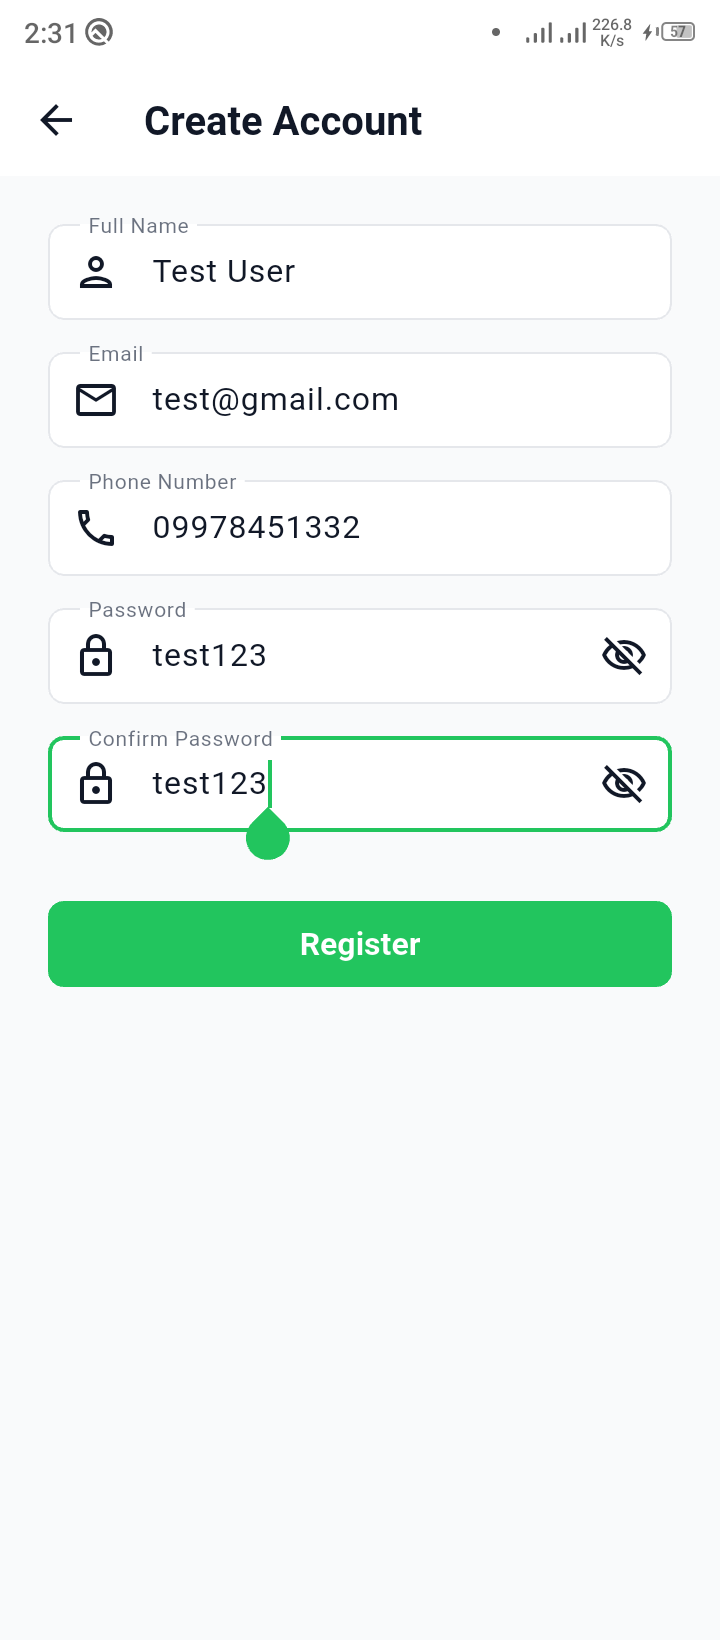
\includegraphics[width=0.45\textwidth]{figures/chapter2/E1U1.png}
    \caption{User Registration Screen Screenshot}
    \label{fig:ui_e1u1}
\end{figure}

\textbf{UI Layout:} Centered form layout with the application logo 
at the top.

\textbf{Fields and Components:} The screen incorporates several key fields and components, including Full Name (input field)., Email Address (input field)., Phone Number (input field)., Password (input field with obscured text)., Register (primary button)., and Login (text link)..

\textbf{Validation Rules:} The system enforces validation rules where email must be in valid format., password must be at least 6 characters., and all fields are required..

\textbf{Navigation Behavior:} Regarding navigation behavior, on successful registration $\rightarrow$ redirect to login., and on failure $\rightarrow$ show error toast..

\subsubsection{Login Screen}

\begin{figure}[H]
    \centering
    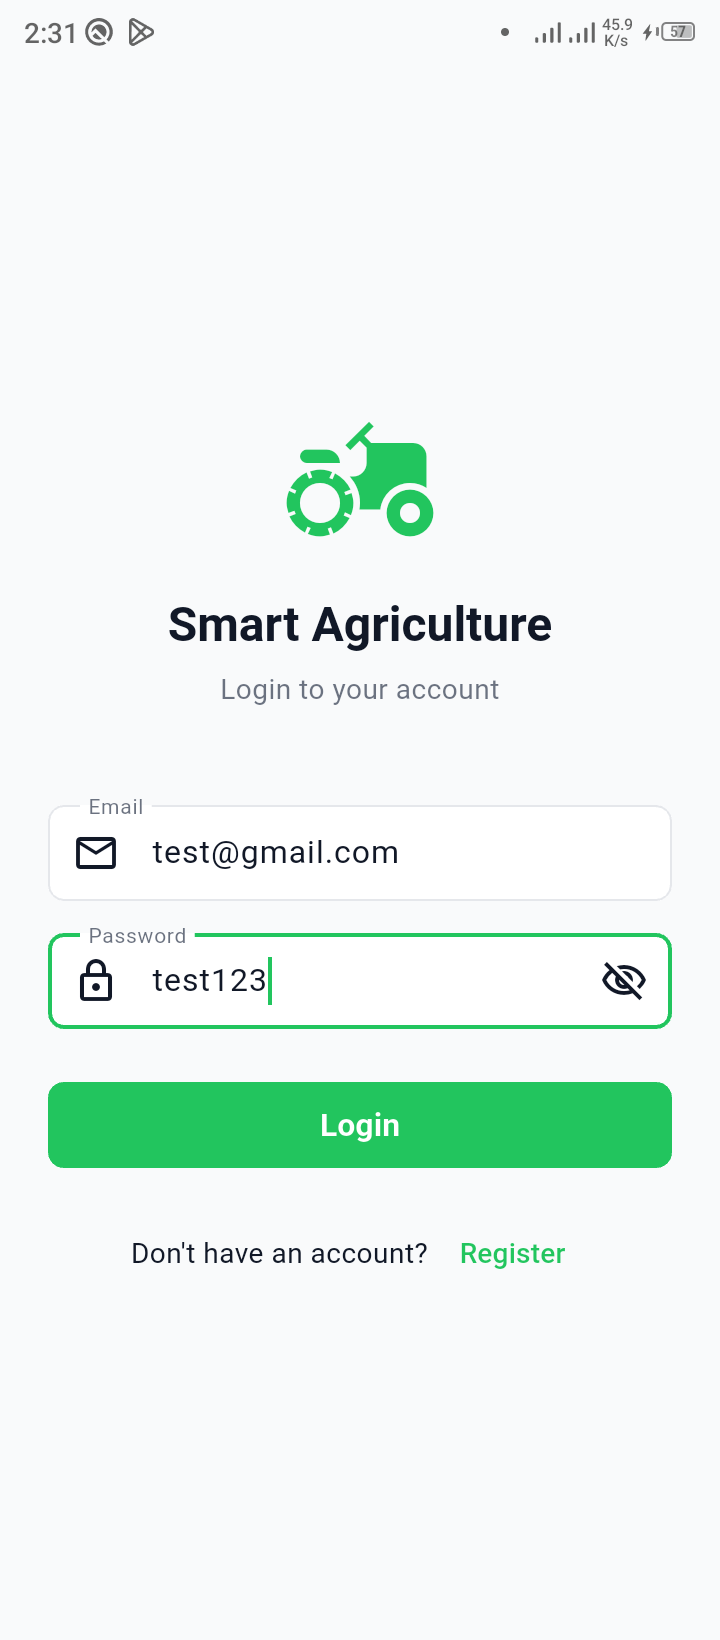
\includegraphics[width=0.45\textwidth]{figures/chapter2/E1U2.png}
    \caption{Login Screen Screenshot}
    \label{fig:ui_e1u2}
\end{figure}

\textbf{UI Layout:} Centered card layout with branding.

\textbf{Fields and Components:} The screen incorporates several key fields and components, including Email Address (input field)., Password (input field)., Login (primary button)., and Forgot Password (link)..

\textbf{Validation Rules:} The system enforces validation rules where email and password cannot be empty..

\textbf{Navigation Behavior:} Regarding navigation behavior, on successful login $\rightarrow$ redirect to dashboard., and on failure $\rightarrow$ show error toast..

\subsubsection{Profile Management Screen}

\begin{figure}[H]
    \centering
    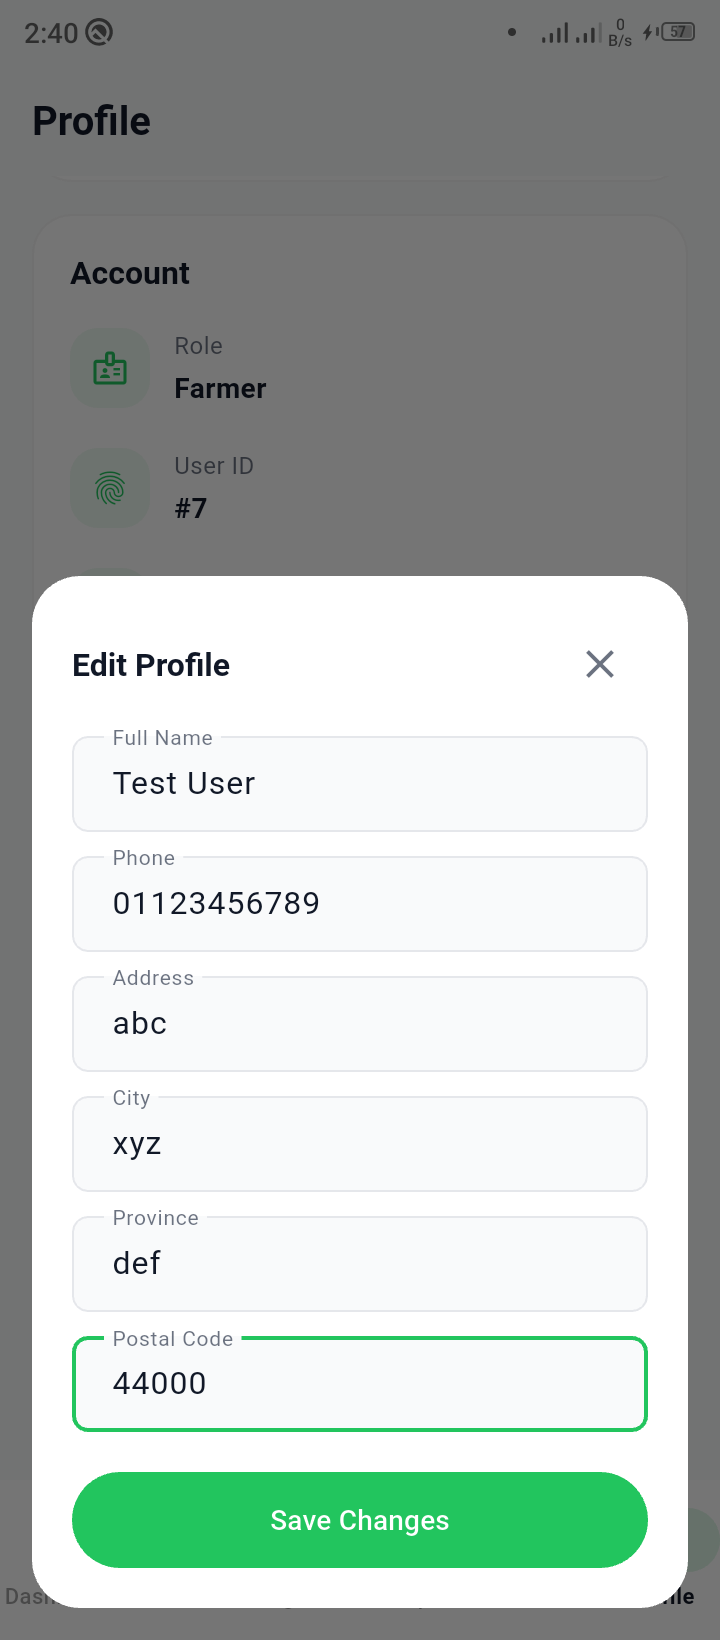
\includegraphics[width=0.45\textwidth]{figures/chapter2/E1U3.png}
    \caption{Profile Management Screen Screenshot}
    \label{fig:ui_e1u3}
\end{figure}

\textbf{UI Layout:} List view of editable user details.

\textbf{Fields and Components:} The screen incorporates several key fields and components, including Profile Picture (avatar)., Name, Email, Phone (editable fields)., Update Profile (button)., and Change Password (button)..

\textbf{Validation Rules:} The system enforces validation rules where valid phone number format., and current password required for password change..

\textbf{Navigation Behavior:} Regarding navigation behavior, on save $\rightarrow$ stay on page with success message..

\subsubsection{Dashboard (Field Overview)}

\begin{figure}[H]
    \centering
    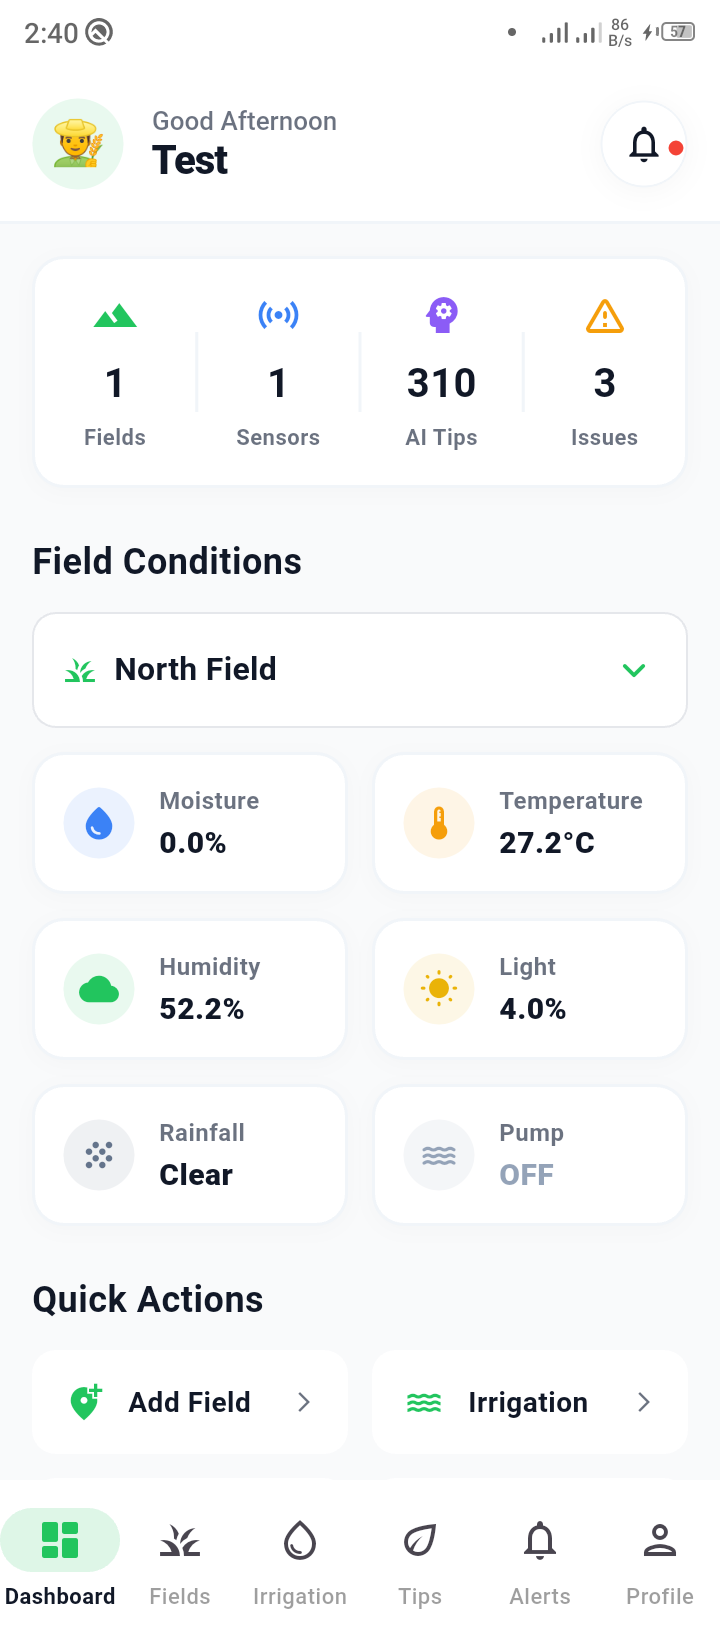
\includegraphics[width=0.45\textwidth]{figures/chapter2/E2U1.png}
    \caption{Dashboard (Field Overview) Screenshot}
    \label{fig:ui_e2u1}
\end{figure}

\textbf{UI Layout:} Grid layout of cards for each registered field 
\cite{kisanvishwa2024}.

\textbf{Fields and Components:} The screen incorporates several key fields and components, including Field Name (header)., Status Indicator (color dot)., Quick Stats (moisture, temp)., and Add New Field (floating action button)..

\textbf{Validation Rules:} There are no specific input validation rules for this screen.

\textbf{Navigation Behavior:} Regarding navigation behavior, tap on field $\rightarrow$ navigate to field details..

\subsubsection{Detailed Sensor Data Screen}

\begin{figure}[H]
    \centering
    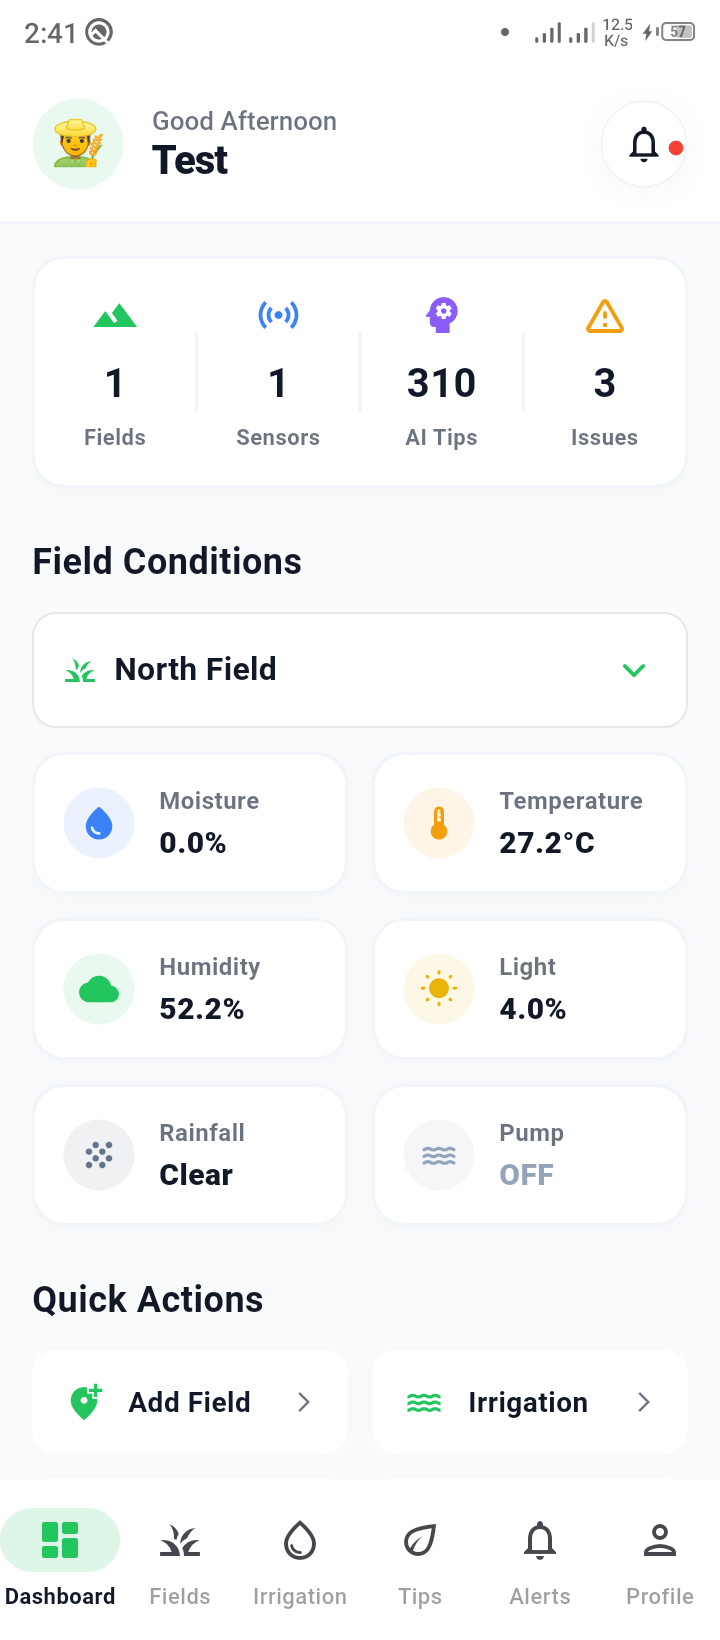
\includegraphics[width=0.45\textwidth]{figures/chapter2/E2U2.png}
    \caption{Detailed Sensor Data Screen Screenshot}
    \label{fig:ui_e2u2}
\end{figure}

\textbf{UI Layout:} Dashboard view with live charts and digital 
readouts.

\textbf{Fields and Components:} The screen incorporates several key fields and components, including Moisture Gauge Chart., Temperature/Humidity Readouts., Last Updated Timestamp., and Refresh (button)..

\textbf{Validation Rules:} The system enforces validation rules where data refreshes automatically every 30 seconds..

\textbf{Navigation Behavior:} Regarding navigation behavior, back button $\rightarrow$ return to field overview..

\subsubsection{Sensor Status Monitoring}

\begin{figure}[H]
    \centering
    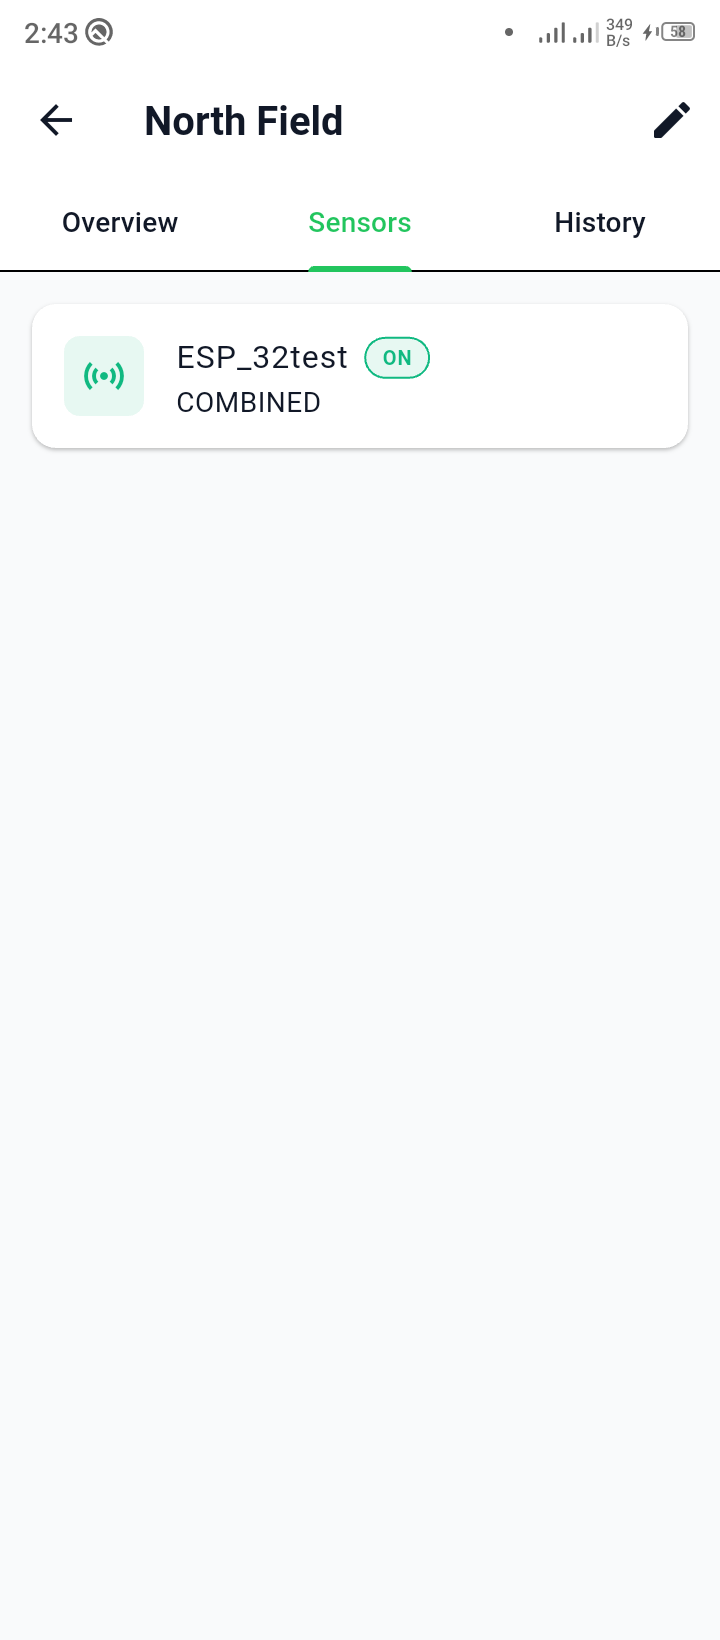
\includegraphics[width=0.45\textwidth]{figures/chapter2/E2U3.png}
    \caption{Sensor Status Monitoring Screenshot}
    \label{fig:ui_e2u3}
\end{figure}

\textbf{UI Layout:} List layout of all sensors and their 
connectivity status.

\textbf{Fields and Components:} The screen incorporates several key fields and components, including Sensor ID (text)., Connection Status (Online/Offline indicator)., and Last Ping Time (timestamp)..

\textbf{Validation Rules:} The system enforces validation rules where status updates based on heartbeat signal..

\textbf{Navigation Behavior:} Regarding navigation behavior, tap on sensor $\rightarrow$ navigate to sensor diagnostics..

\subsubsection{Manual Irrigation Control}

\begin{figure}[H]
    \centering
    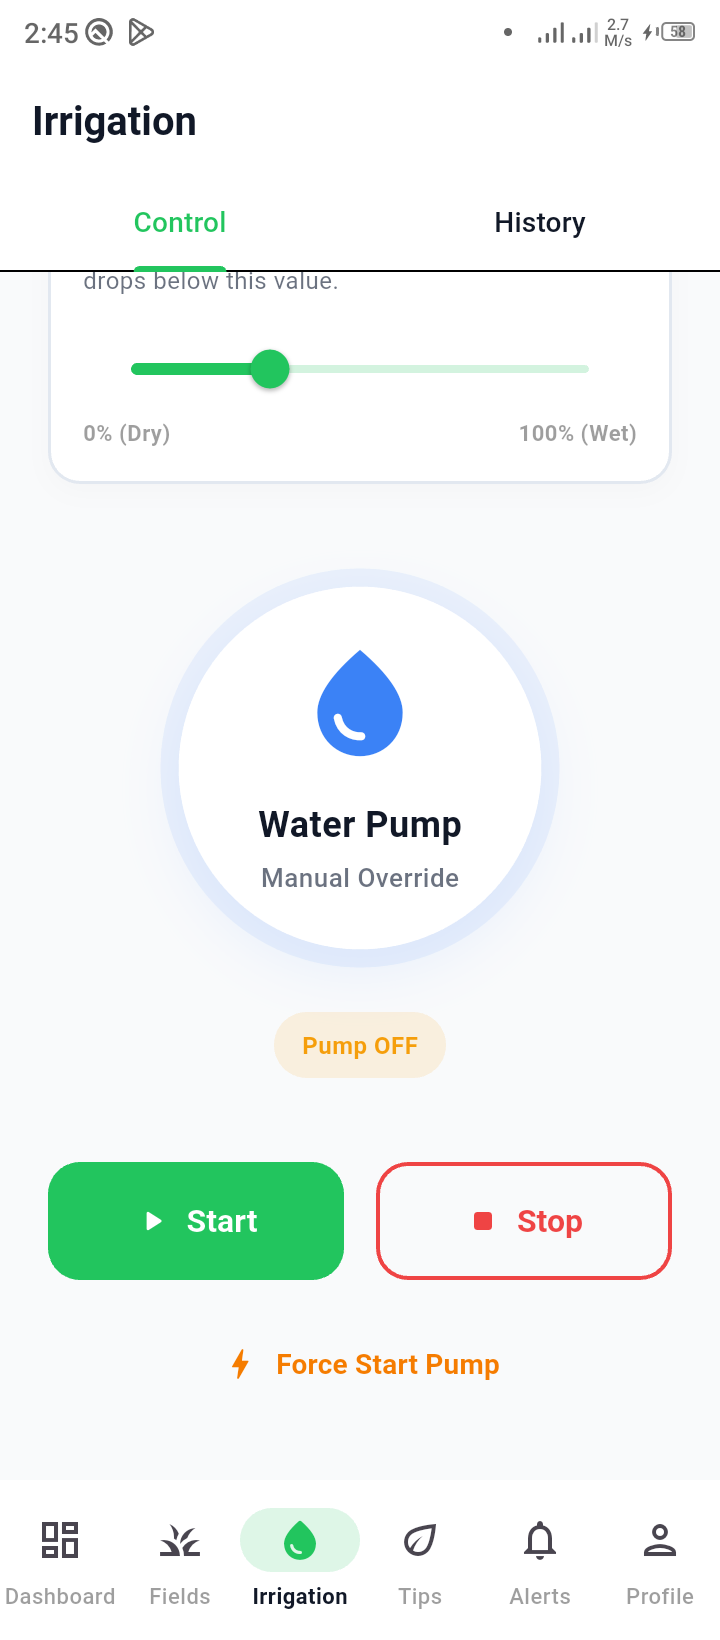
\includegraphics[width=0.45\textwidth]{figures/chapter2/E3U1.png}
    \caption{Manual Irrigation Control Screenshot}
    \label{fig:ui_e3u1}
\end{figure}

\textbf{UI Layout:} Card layout with prominent toggle switches.

\textbf{Fields and Components:} The screen incorporates several key fields and components, including Pump Power (toggle switch)., Field Selector (dropdown)., Pump Status (indicator)., and Start/Stop Timer (input)..

\textbf{Validation Rules:} The system enforces validation rules where pump cannot start if auto-irrigation is active..

\textbf{Navigation Behavior:} Regarding navigation behavior, toggle switch $\rightarrow$ sends immediate api request to esp32..

\subsubsection{Auto-Irrigation Settings}

\begin{figure}[H]
    \centering
    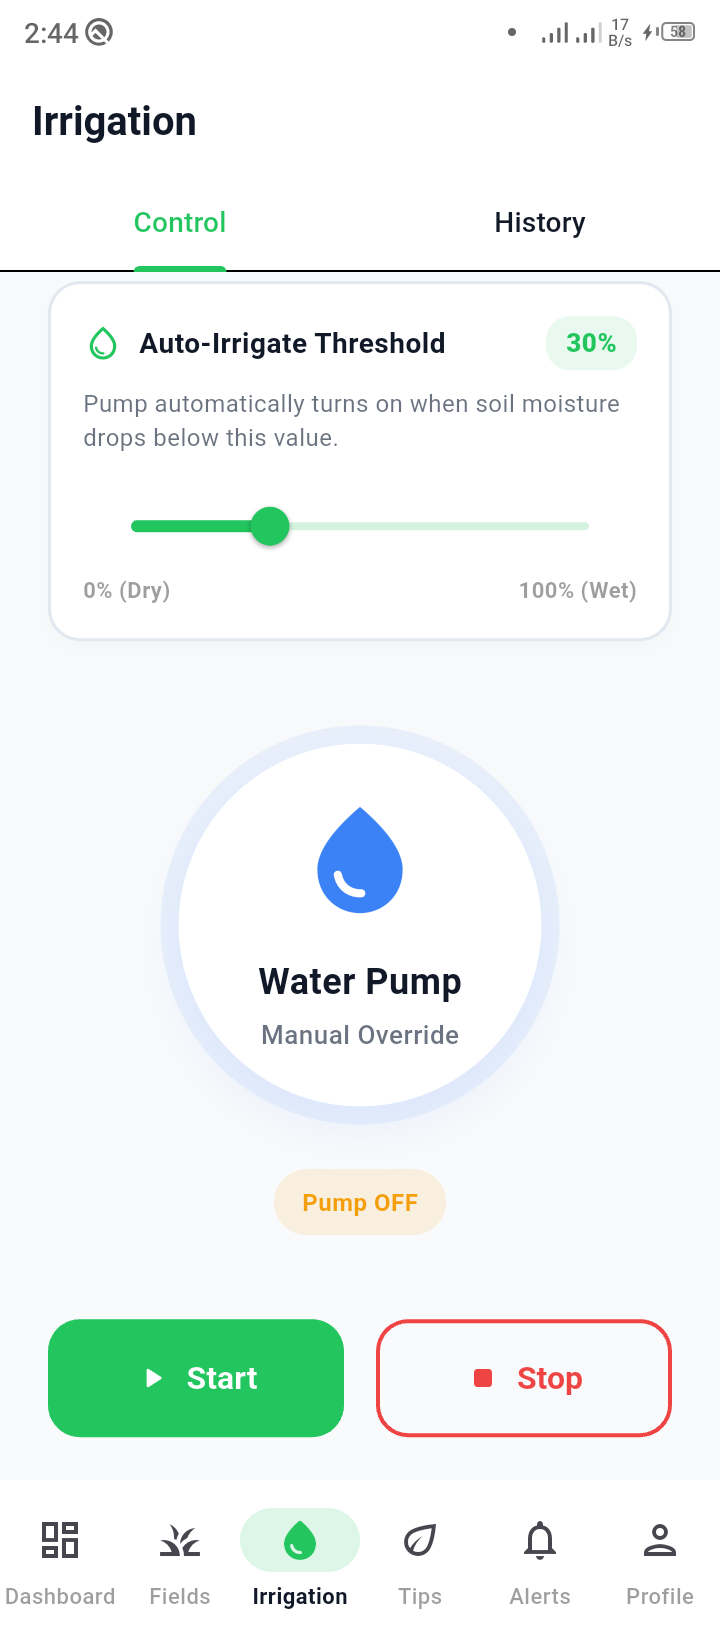
\includegraphics[width=0.45\textwidth]{figures/chapter2/E3U2.png}
    \caption{Auto-Irrigation Settings Screenshot}
    \label{fig:ui_e3u2}
\end{figure}

\textbf{UI Layout:} Settings form with sliders and checkboxes.

\textbf{Fields and Components:} The screen incorporates several key fields and components, including Enable Auto-Irrigation (checkbox)., Moisture Threshold (slider 0-100\%)., and Save Configuration (button)..

\textbf{Validation Rules:} The system enforces validation rules where threshold must be between 10\% and 90\%..

\textbf{Navigation Behavior:} Regarding navigation behavior, save $\rightarrow$ updates device settings and returns to previous screen..

\subsubsection{Irrigation Logs}

\begin{figure}[H]
    \centering
    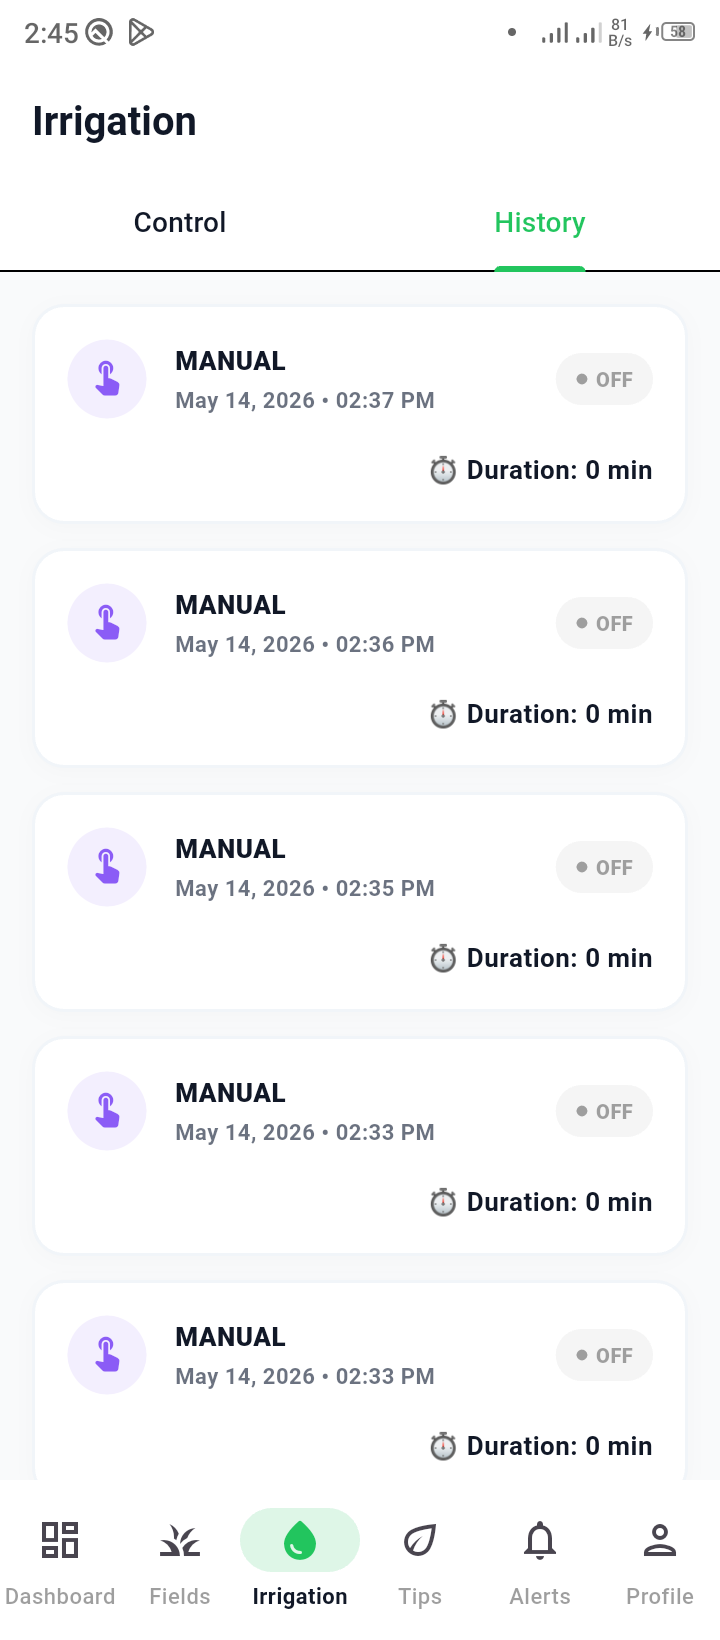
\includegraphics[width=0.45\textwidth]{figures/chapter2/E3U3.png}
    \caption{Irrigation Logs Screenshot}
    \label{fig:ui_e3u3}
\end{figure}

\textbf{UI Layout:} Chronological list view of past irrigation 
events.

\textbf{Fields and Components:} The screen incorporates several key fields and components, including Date \& Time (text)., Duration (text)., Trigger Type (Manual/Auto label)., and Water Volume Used (stats)..

\textbf{Validation Rules:} The system enforces validation rules where logs are read-only..

\textbf{Navigation Behavior:} Regarding navigation behavior, filter button $\rightarrow$ opens date range picker..

\subsubsection{Crop Recommendation Form}

\begin{figure}[H]
    \centering
    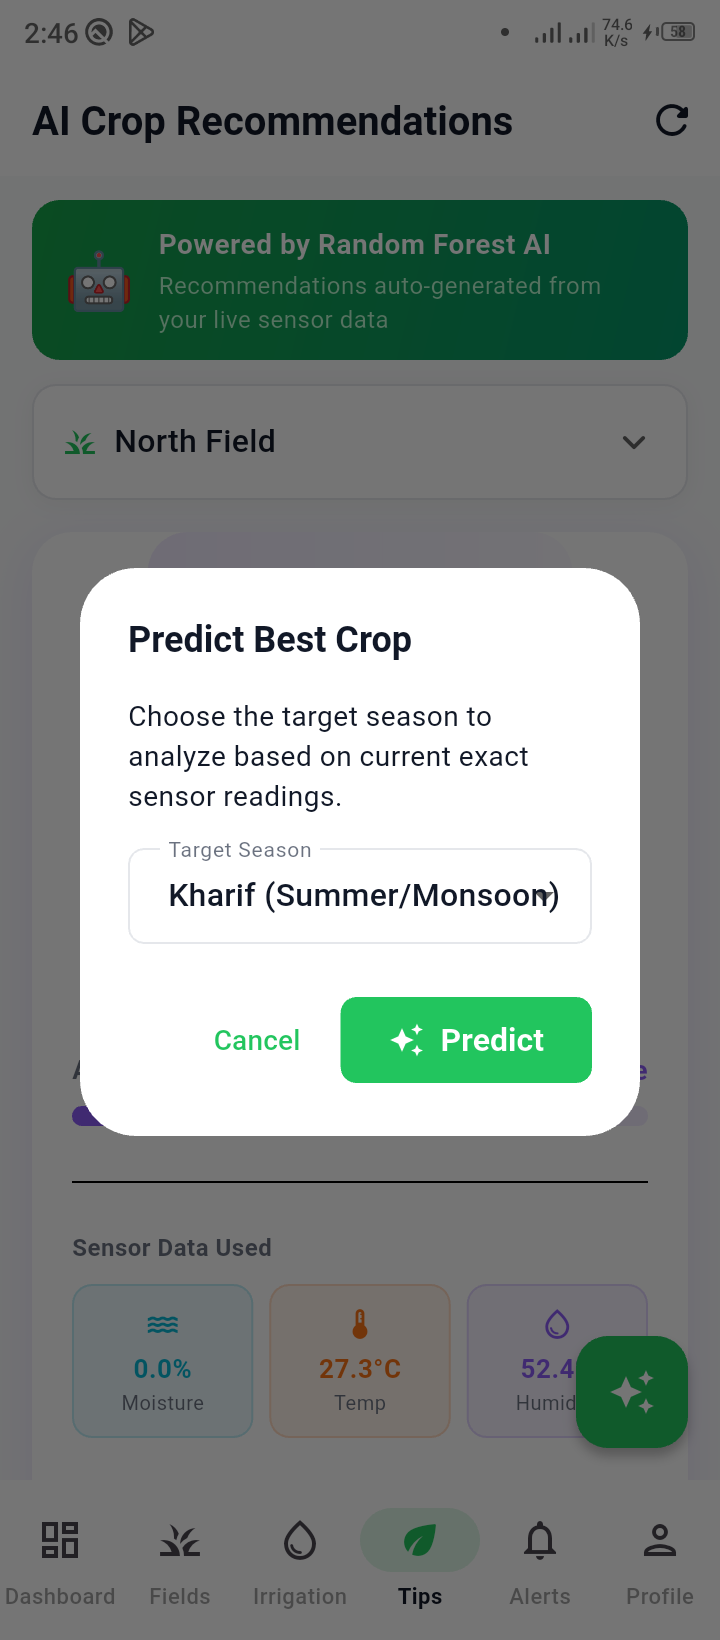
\includegraphics[width=0.45\textwidth]{figures/chapter2/E4U1.png}
    \caption{Crop Recommendation Form Screenshot}
    \label{fig:ui_e4u1}
\end{figure}

\textbf{UI Layout:} Form layout with selection dropdowns.

\textbf{Fields and Components:} The screen incorporates several key fields and components, including Field Selector (dropdown)., Soil Type (dropdown)., Season (dropdown)., and Analyze Conditions (button)..

\textbf{Validation Rules:} The system enforces validation rules where all fields must be selected before analysis..

\textbf{Navigation Behavior:} Regarding navigation behavior, analyze $\rightarrow$ navigates to recommendation result screen..

\subsubsection{Recommendation Result}

\begin{figure}[H]
    \centering
    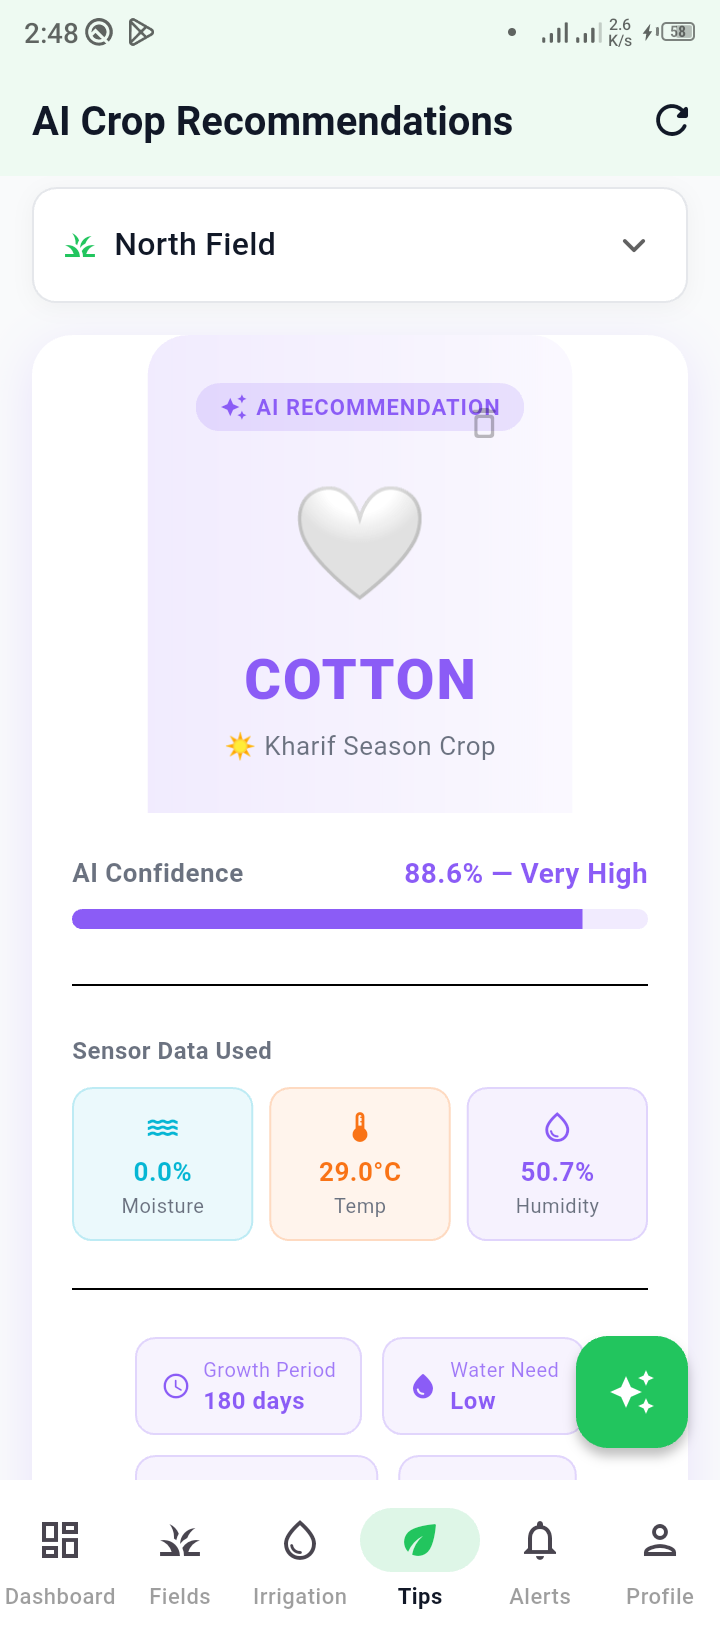
\includegraphics[width=0.45\textwidth]{figures/chapter2/E4U2.png}
    \caption{Recommendation Result Screenshot}
    \label{fig:ui_e4u2}
\end{figure}

\textbf{UI Layout:} Result card with AI insights and confidence 
score.

\textbf{Fields and Components:} The screen incorporates several key fields and components, including Recommended Crop Name (large text)., Confidence Score (progress circle)., Expected Yield (text)., Accept (button)., and Reject (button)..

\textbf{Validation Rules:} The system enforces validation rules where confidence score must be loaded before showing actions..

\textbf{Navigation Behavior:} Regarding navigation behavior, accept $\rightarrow$ updates field crop details., and reject $\rightarrow$ returns to form..

\subsubsection{Accepted Recommendation Details}

\begin{figure}[H]
    \centering
    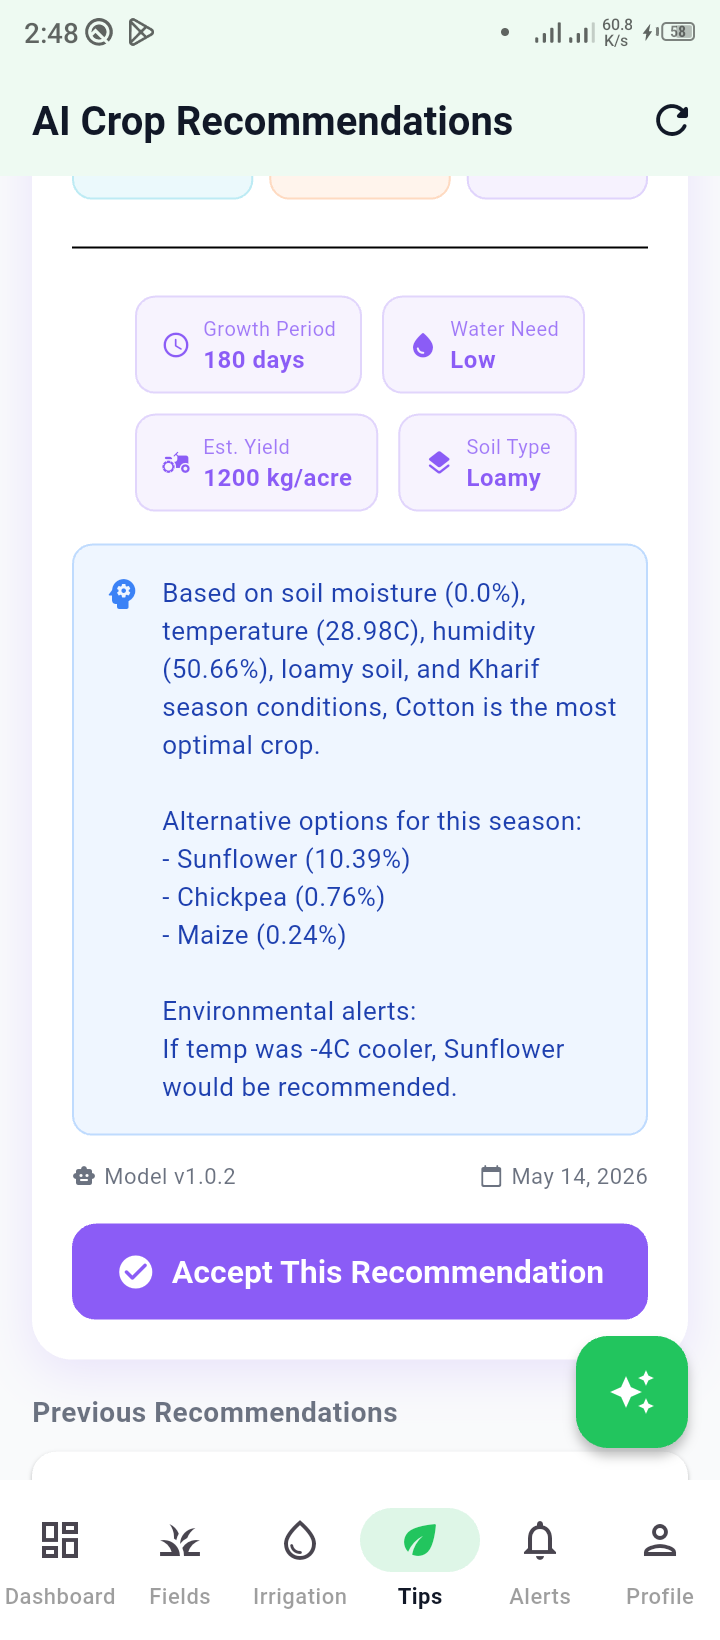
\includegraphics[width=0.45\textwidth]{figures/chapter2/E4U3.png}
    \caption{Accepted Recommendation Details Screenshot}
    \label{fig:ui_e4u3}
\end{figure}

\textbf{UI Layout:} Detail view showing accepted crop parameters.

\textbf{Fields and Components:} The screen incorporates several key fields and components, including Crop Growth Stage (timeline)., Watering Requirements (stats)., and Harvest Estimate (date)..

\textbf{Validation Rules:} The system enforces validation rules where data bound to the accepted crop profile..

\textbf{Navigation Behavior:} Regarding navigation behavior, back $\rightarrow$ navigates to dashboard..

\subsubsection{Critical Alert Notification}

\begin{figure}[H]
    \centering
    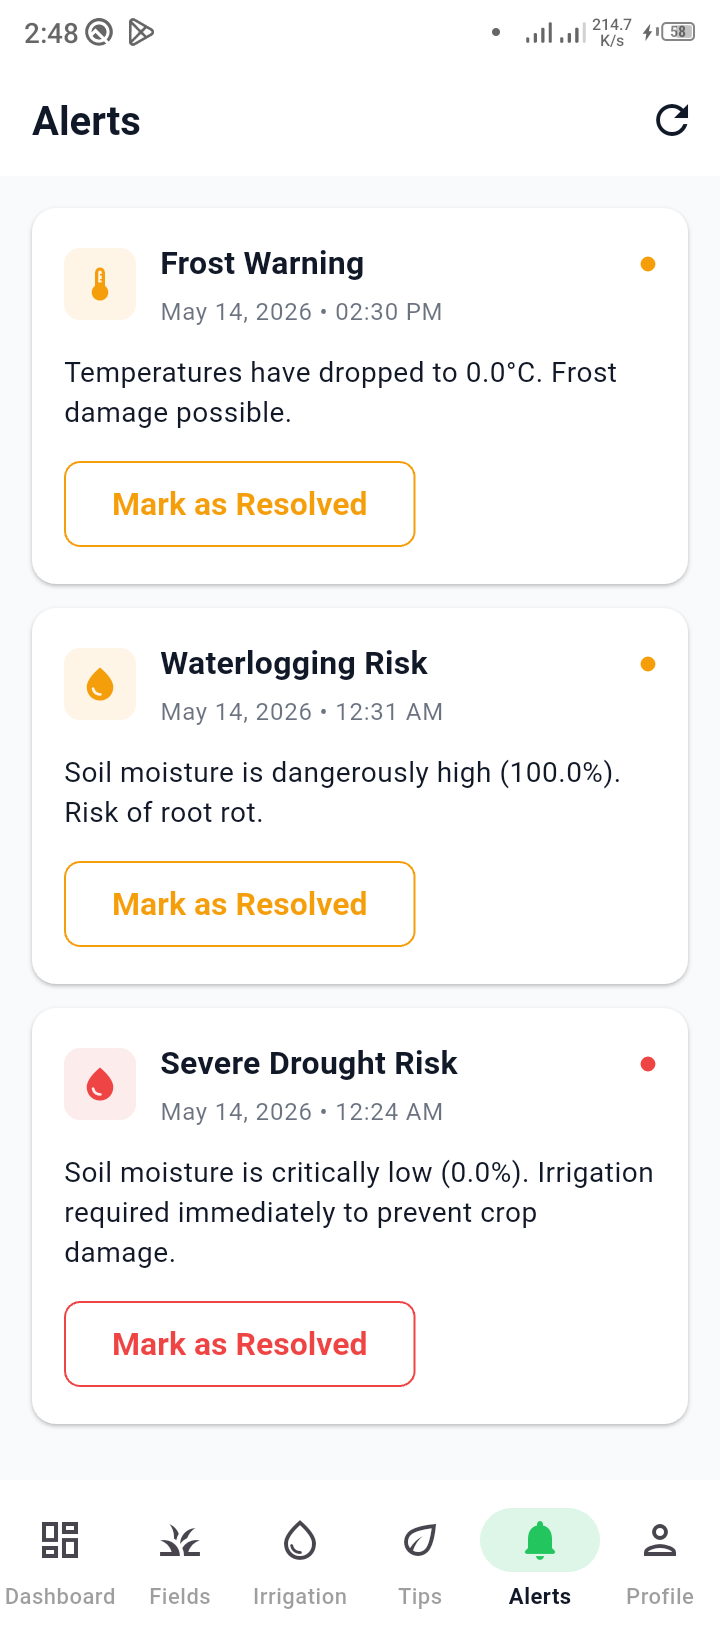
\includegraphics[width=0.45\textwidth]{figures/chapter2/E5U1.png}
    \caption{Critical Alert Notification Screenshot}
    \label{fig:ui_e5u1}
\end{figure}

\textbf{UI Layout:} Popup modal or banner for urgent attention.

\textbf{Fields and Components:} The screen incorporates several key fields and components, including Warning Icon., Alert Title (bold text)., Action Required (description)., Acknowledge (button)., and Go to Field (button)..

\textbf{Validation Rules:} The system enforces validation rules where modal cannot be dismissed without acknowledgement..

\textbf{Navigation Behavior:} Regarding navigation behavior, go to field $\rightarrow$ navigates to field details., and acknowledge $\rightarrow$ dismisses modal..

\subsubsection{Alert Center}

\begin{figure}[H]
    \centering
    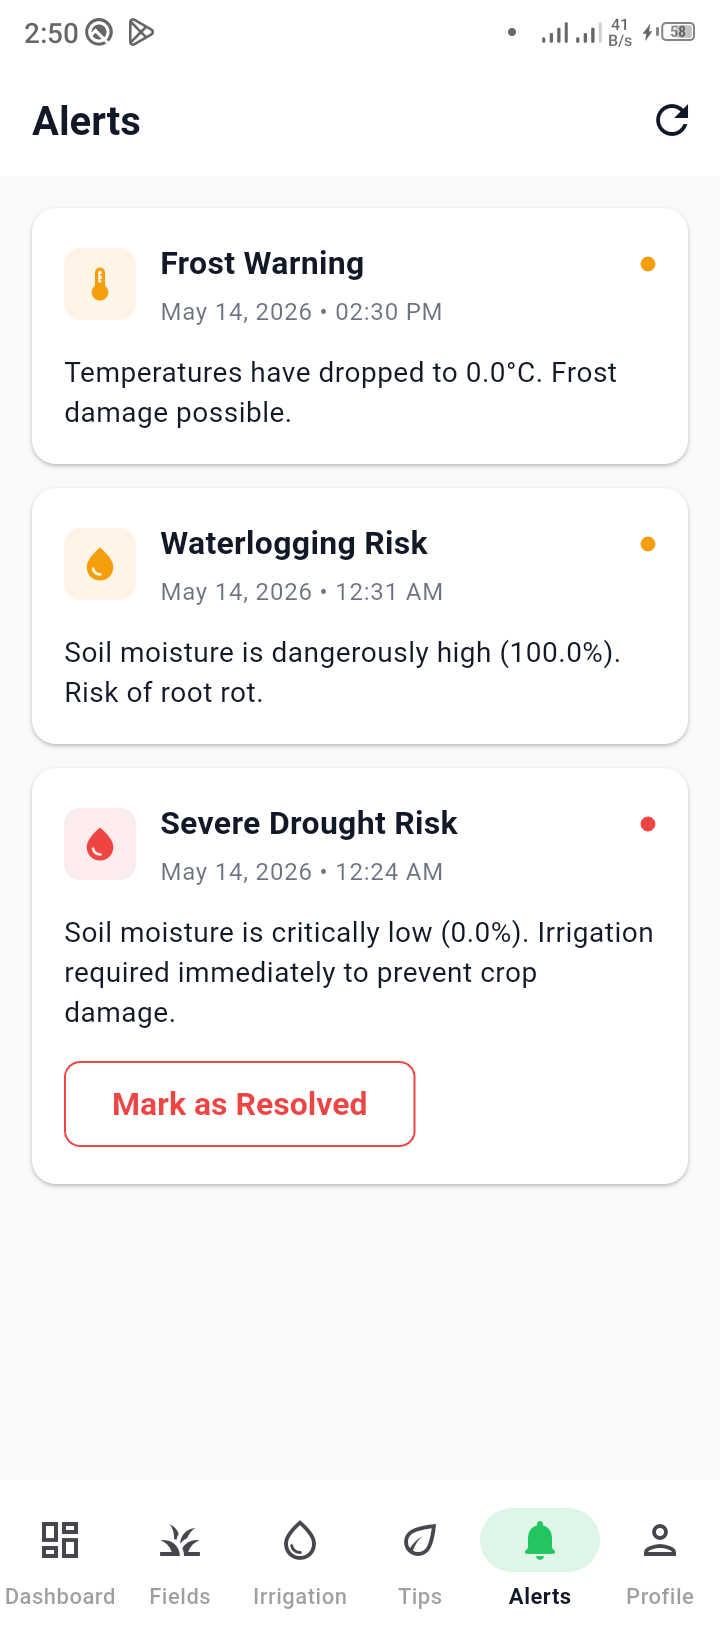
\includegraphics[width=0.45\textwidth]{figures/chapter2/E5U2.png}
    \caption{Alert Center Screenshot}
    \label{fig:ui_e5u2}
\end{figure}

\textbf{UI Layout:} List view of active and recent notifications.

\textbf{Fields and Components:} The screen incorporates several key fields and components, including Unread Badge (count indicator)., Alert Items (cards)., Mark All Read (button)., and Filter (dropdown)..

\textbf{Validation Rules:} The system enforces validation rules where unread items highlighted with different background color..

\textbf{Navigation Behavior:} Regarding navigation behavior, tap alert $\rightarrow$ opens alert details or relevant screen..

\subsubsection{Resolved Alerts History}

\begin{figure}[H]
    \centering
    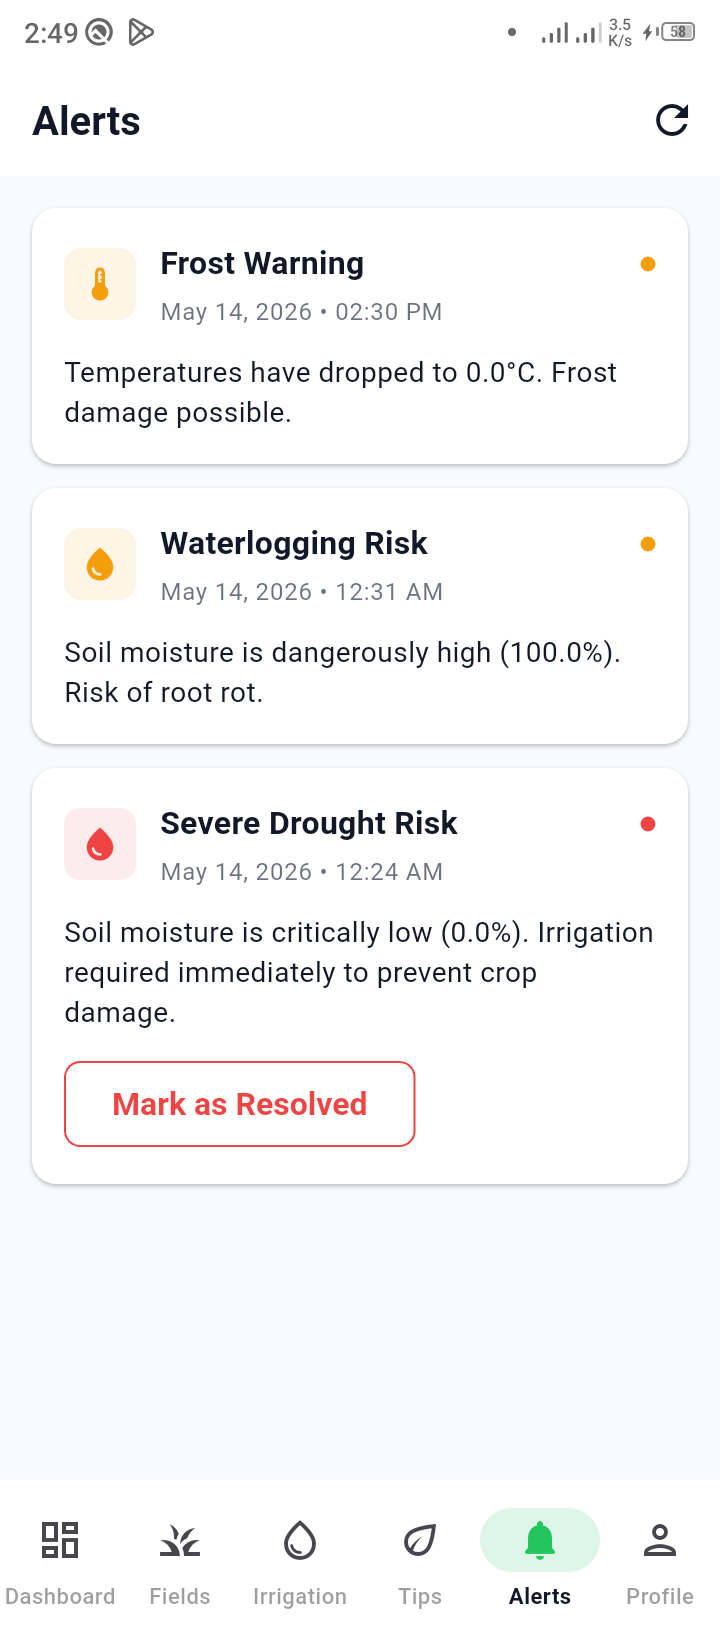
\includegraphics[width=0.45\textwidth]{figures/chapter2/E5U3.png}
    \caption{Resolved Alerts History Screenshot}
    \label{fig:ui_e5u3}
\end{figure}

\textbf{UI Layout:} Archived list view of past issues.

\textbf{Fields and Components:} The screen incorporates several key fields and components, including Resolved Date (timestamp)., Original Issue (text)., and Resolution Action (text)..

\textbf{Validation Rules:} The system enforces validation rules where read-only historical data..

\textbf{Navigation Behavior:} Regarding navigation behavior, swipe $\rightarrow$ delete from history (optional)..

\subsubsection{Weekly Trend Graph}

\begin{figure}[H]
    \centering
    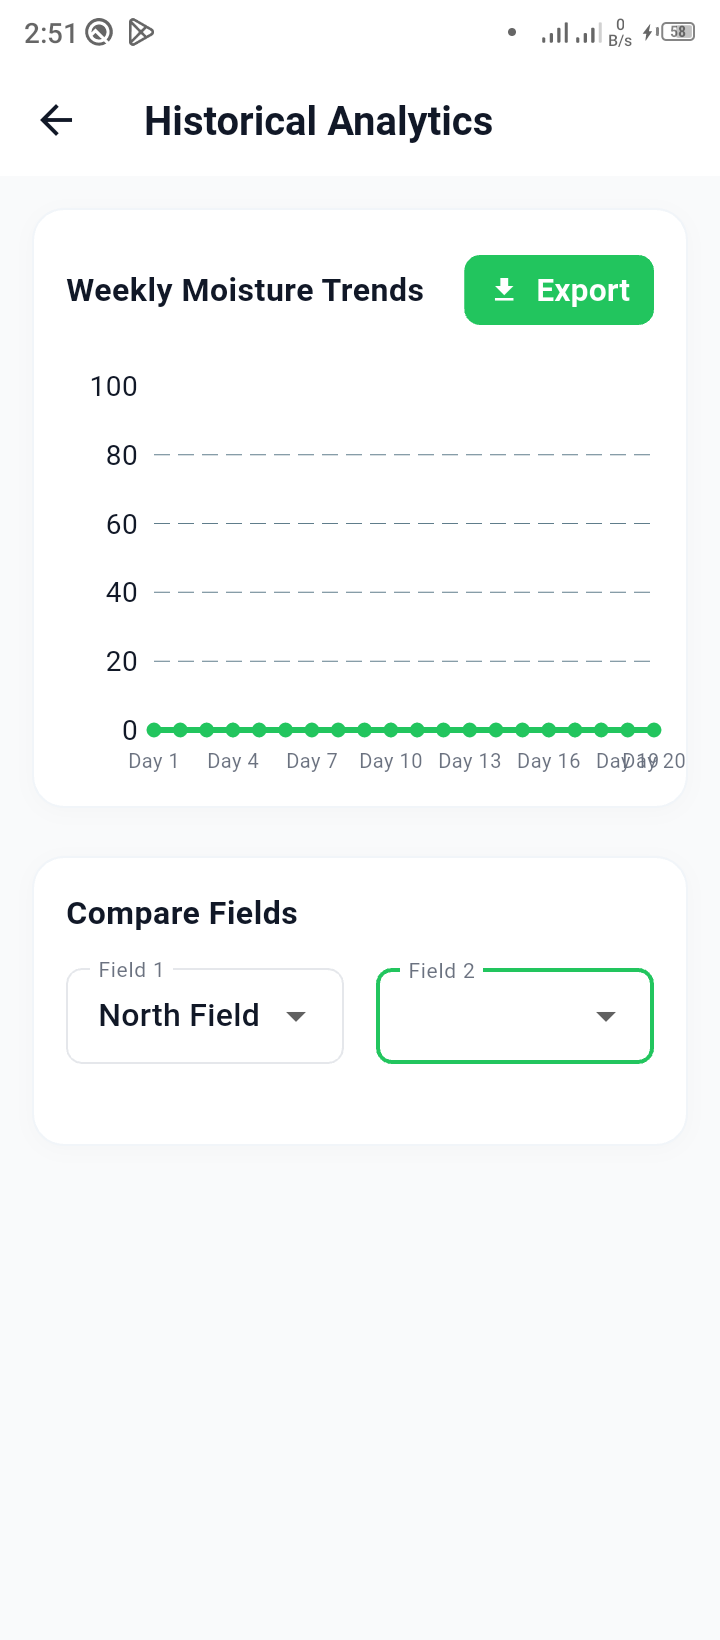
\includegraphics[width=0.45\textwidth]{figures/chapter2/E6U1.png}
    \caption{Weekly Trend Graph Screenshot}
    \label{fig:ui_e6u1}
\end{figure}

\textbf{UI Layout:} Full-width chart container with interactive 
tooltips.

\textbf{Fields and Components:} The screen incorporates several key fields and components, including Line Chart (moisture over time)., Time Range Selector (tabs: 1W, 1M, 3M)., and Data Points (tooltips)..

\textbf{Validation Rules:} The system enforces validation rules where chart re-renders when time range changes..

\textbf{Navigation Behavior:} Regarding navigation behavior, pinch/zoom $\rightarrow$ interacts with chart data..

\subsubsection{Data Export Screen}

\begin{figure}[H]
    \centering
    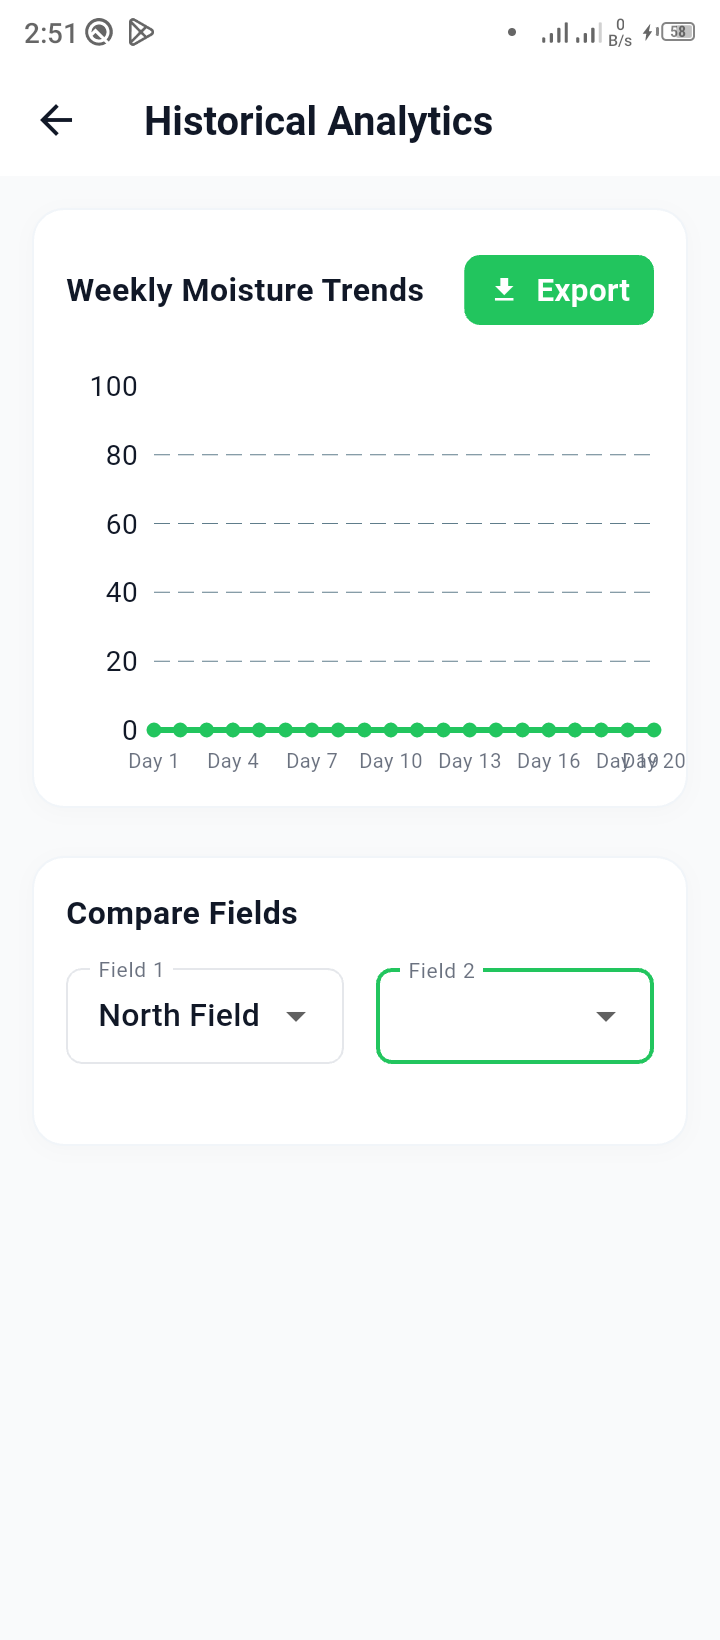
\includegraphics[width=0.45\textwidth]{figures/chapter2/E6U2.png}
    \caption{Data Export Screen Screenshot}
    \label{fig:ui_e6u2}
\end{figure}

\textbf{UI Layout:} Configuration form for report generation.

\textbf{Fields and Components:} The screen incorporates several key fields and components, including Date Range Picker (inputs)., Data Type (checkboxes: Moisture, Irrigation)., Format Selector (CSV/PDF)., and Generate Report (button)..

\textbf{Validation Rules:} The system enforces validation rules where end date cannot be before start date..

\textbf{Navigation Behavior:} Regarding navigation behavior, generate $\rightarrow$ shows loading spinner, then download prompt..

\subsubsection{Field Comparison View}

\begin{figure}[H]
    \centering
    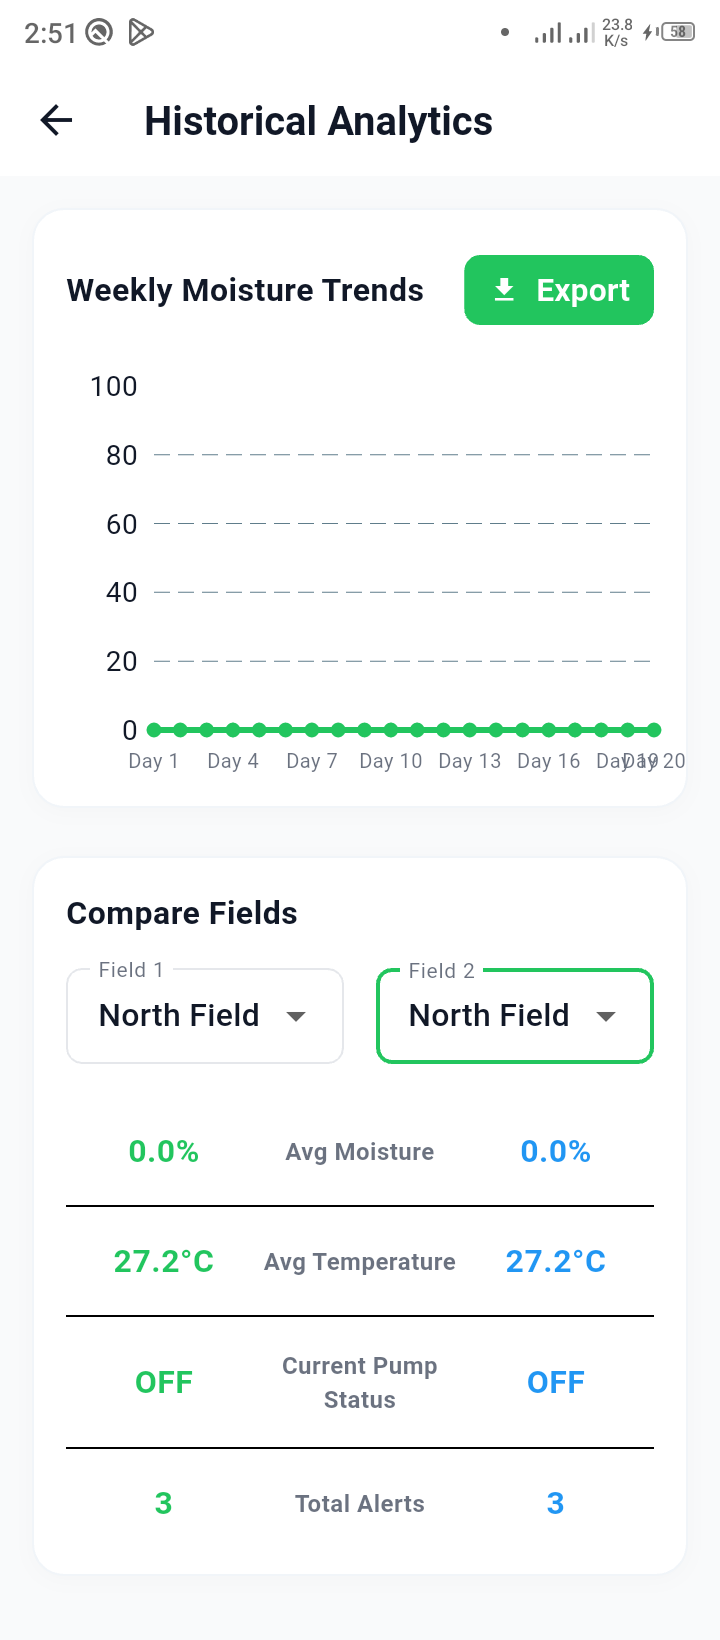
\includegraphics[width=0.45\textwidth]{figures/chapter2/E6U3.png}
    \caption{Field Comparison View Screenshot}
    \label{fig:ui_e6u3}
\end{figure}

\textbf{UI Layout:} Side-by-side split view or comparative bar 
charts.

\textbf{Fields and Components:} The screen incorporates several key fields and components, including Field A Selector (dropdown)., Field B Selector (dropdown)., Comparative Bar Charts., and Metric Highlights (cards)..

\textbf{Validation Rules:} The system enforces validation rules where field a and field b cannot be the same..

\textbf{Navigation Behavior:} Regarding navigation behavior, change selector $\rightarrow$ instantly updates charts..

\subsection{Traceability Matrix}

The traceability matrix maps epics to user stories, test cases, and 
UI screens to ensure full coverage of requirements and proper 
validation \cite{tahir2019traceability}.

{
\small
\begin{longtable}{|p{2cm}|p{4cm}|p{3cm}|p{3cm}|}
\caption{Traceability Matrix}
\label{tab:traceability} \\
\hline
\textbf{Epic} & \textbf{User Story} & \textbf{Test Case} & 
\textbf{UI Screen} \\ \hline
\endfirsthead

\multicolumn{4}{c}%
{{\bfseries \tablename\ \thetable{} -- Continued from previous 
page}} \\
\hline
\textbf{Epic} & \textbf{User Story} & \textbf{Test Case} & 
\textbf{UI Screen} \\ \hline
\endhead

\hline \multicolumn{4}{|r|}{{Continued on next page...}} \\ \hline
\endfoot

\hline
\endlastfoot

E1 (Auth) & E1-US1 (Register) & TC-E1-US1-01 & Login Screen 
(Register) \\ \hline
E1 (Auth) & E1-US2 (Login) & TC-E1-US2-01 & Login Screen \\ \hline
E1 (Auth) & E1-US3 (Profile) & N/A (Standard Update) & Settings / 
Profile Page \\ \hline

E2 (Monitoring) & E2-US1 (Field Overview) & N/A (Visual Check) & 
Dashboard \\ \hline
E2 (Monitoring) & E2-US2 (Sensor Detail) & TC-E2-US2-01 & Detailed 
Sensor Data Page \\ \hline
E2 (Monitoring) & E2-US3 (Status) & N/A (Status Check) & Dashboard 
/ Sensor Page \\ \hline

E3 (Irrigation) & E3-US1 (Manual) & TC-E3-US1-01 & Irrigation 
Control Panel \\ \hline
E3 (Irrigation) & E3-US2 (Auto) & TC-E3-US2-01 & Irrigation Control 
Panel \\ \hline
E3 (Irrigation) & E3-US3 (Logs) & N/A (Log Check) & Detailed Sensor 
Data Page (History Tab) \\ \hline

E4 (AI) & E4-US1 (Request Rec) & TC-E4-US1-01 & AI Crop 
Recommendation Screen \\ \hline
E4 (AI) & E4-US2 (Confidence) & N/A (Visual Check) & AI Crop 
Recommendation Screen \\ \hline
E4 (AI) & E4-US3 (Accept) & N/A (State Change) & AI Crop 
Recommendation Screen \\ \hline

E5 (Alerts) & E5-US1 (Critical) & TC-E5-US1-01 & Alerts \& 
Notifications Screen \\ \hline
E5 (Alerts) & E5-US2 (Unread) & N/A (Badge Check) & Dashboard 
(Alert Icon) \\ \hline
E5 (Alerts) & E5-US3 (Resolve) & N/A (Action Check) & Alerts \& 
Notifications Screen \\ \hline

E6 (Analytics) & E6-US1 (Trends) & TC-E6-US1-01 & Detailed Sensor 
Data Page (History) \\ \hline
E6 (Analytics) & E6-US2 (Export) & N/A (Download) & Settings / 
Profile Page \\ \hline
E6 (Analytics) & E6-US3 (Compare) & N/A (Multi-view) & Dashboard 
(Comparison View) \\ \hline
\end{longtable}
}

\setcounter{chapter}{2}